% !TeX program = pdflatex
% !TeX spellcheck = en_GB
% !TeX TXS-program:bibliography = txs:///bibtex

\documentclass[Master, ngerman, UKenglish]{scrbook}
%------------------------------------------------------------------------------
% This file contains a skeleton thesis for
% a Physics or Astronomy Institute in the University of Bonn

% Specify the thesis type as an option: PhD, Master, Diplom, Bachelor
% Specify the thesis stage as an option: Draft (default), Submit, Final, PILibrary

% Specify the language(s) in the class and then use babel.
% If you need more than one language, give the default language last,
% e.g. ngerman, UKenglish for a thesis in British (UK) English where you want
% to be able to set the language to German for some part of it.

%------------------------------------------------------------------------------
% Pass TeX Live version to the package 
% Use command pdflatex --version to find out which version you are running
% Add option backref=false when your thesis is ready to turn off back-referencing
% in your bibliography
\usepackage[texlive=2018,backend=bibtex,backref=False,Master,Submit]{ubonn-thesis}
% Adjustments to standard biblatex style
\usepackage{ubonn-biblatex}

% Glossary package
% \usepackage[acronym,toc,nosuper]{glossaries}
% TikZ packages and libraries
% \usepackage{tikz}
% \usepackage{tikz-3dplot}
% \usepackage{pgfplots}
% \usetikzlibrary{positioning,shapes,arrows}
% \usetikzlibrary{decorations.pathmorphing}
% \usetikzlibrary{decorations.markings}
\usepackage{graphicx}
\usepackage{multirow}
\usepackage{import}
\usepackage{pgf}
\usepackage{pgfplots}
%\pgfplotsset{compat=newest}
\usepackage{thesis_defs}
\usepackage{xcolor}
\definecolor{mygray}{rgb}{211,211,211}
\usepackage{array}
\usepackage{eurosym}
\newcolumntype{C}[1]{>{\centering\arraybackslash}p{#1}}
\newcommand\mc[1]{\multicolumn{1}{c}{#1}}
\usepackage{listings}
\lstdefinestyle{cpp}{
	language=C++,
	backgroundcolor=\color{lightgray},
	frame=none, % draw a frame at the top and bottom of the code block
	tabsize=2, % tab space width
	commentstyle=\color{darkgreen}, % comment color
	keywordstyle=\color{blue}, % keyword color
	stringstyle=\color{red}, % string color
 morestring=[b]",
	% showstringspaces=false, % don't mark spaces in strings
	%numbers=right, % display line numbers on the left
}
\lstnewenvironment{codecpp}[1][]%
{\\\noindent\minipage{\textwidth}\medskip 
	\lstset{language=C++,
		basicstyle=\footnotesize,
		keywordstyle=\color{blue}\ttfamily,
		tabsize=2,
		breaklines=true,
		showstringspaces=false,
		stringstyle=\color{red}\ttfamily,
		commentstyle=\color{darkgreen}\ttfamily,
		morecomment=[l][\color{darkgreen}]{//},
		morecomment=[l][\color{green}]{//<},
		frame=none,#1,
		backgroundcolor=\color{lightgray}}}{\endminipage\vspace{1cm}\\}


%\usepackage{subfigure}
\usepackage{nicefrac}
\usepackage{graphbox}
\usepackage[bottom]{footmisc}
\usepackage{multicol}
%\usepackage{cite}

%------------------------------------------------------------------------------
% Instead of colouring links, cites, table of contents etc.
% put them in a coloured box for the screen version.
% This is probably a good idea when you print your thesis.
% \hypersetup{colorlinks=false,
% linkbordercolor=blue,citebordercolor=magenta,urlbordercolor=darkgreen
% }

%------------------------------------------------------------------------------
% When writing your thesis it is often helpful to have the date and
% time in the output file. Comment this out for the final version.
%\ifoot[\today{} \thistime]{\today{} \thistime}

% In order to check if your labels are referenced try the refcheck package
%\usepackage{refcheck}

%------------------------------------------------------------------------------
% biblatex is included by ubonn-thesis. Look there for the settings used.
% See the options for settings that can be changed easily.
% For further changes copy the \RequirePackage[...]{biblatex} here
% and include ubonn-thesis with the option biblatex=false.

% Specify the bibliography files here and not at the end!
% Use standard_refs-bibtex if you use bibtex or bibtex8
% and standard_refs-if you use biber
\addbibresource{bib/thesis_refs_1.bib}
%\addbibresource{bib/standard_refs-biber.bib}
%\bibliography{./thesis_refs,../refs/standard_refs-bibtex,./bib/thesis_refs}
%\bibliographystyle{../refs/atlasBibStyleWithTitle.bst}
%------------------------------------------------------------------------------
% The following definitions are used to produce the title pages
% needed at various stages
\newcommand{\thesistitle}{Development of a New Revision for Floating, High-Voltage Picoamperemeters}
\newcommand*{\thesisauthor}{Florian Rössing}
\newcommand*{\thesistown}{Place of birth}
\renewcommand*{\InstituteName}{\HISKP}
\renewcommand*{\inInstitute}{\inHISKP}
\renewcommand*{\InstituteAddress}{\HISKPaddress}
% Adjust \thesisreferee...text depending on male/female referee
\newcommand*{\thesisrefereeonetext}{1.\ Gutachter}
\newcommand*{\thesisrefereeone}{Prof.\ Dr.\ Bernhard Ketzer}
\newcommand*{\thesisrefereetwotext}{2.\ Gutachter}
\newcommand*{\thesisrefereetwo}{PD Dr.\ Paul-Dieter Eversheim }
% Date when thesis was submitted (Master/Diplom)
% Year or Month, Year when thesis was submitted (PhD)
\newcommand*{\thesissubmit}{XX.YY.2018}
%\part{title}% \newcommand*{\thesissubmit}{Month 2018}
% Date of thesis examination (PhD)
\newcommand*{\thesispromotion}{XX.YY.2018}
% Month and year of the final printed version of the thesis
\newcommand*{\thesismonth}{06}
\newcommand*{\thesisyear}{2020}
\newcommand*{\thesisnumber}{BONN-IR-2018-XXX}
\DeclareSIUnit{\euro}{€}
\DeclareSIUnit{\bit}{-bit}
\DeclareSIUnit{\sqhz}{$\sqrt{\text{\hertz}}$}
\DeclareSIUnit{\amp}{\ampere}
\DeclareSIUnit{\sps}{sps}



%----------------------------------------------------------------------
\usepackage[nohyperlinks]{acronym}

\newcommand{\pin}[1]{\textbf{#1}}
\newcommand{\file}[1]{\textit{#1}}
\newcommand{\function}[1]{#1}
\newcommand{\code}[1]{\textit{#1}}
%------------------------------------------------------------------------------
% The abstract is only needed for the printed version and should be in
% English regardless of the language of the thesis
\newcommand{\thesisabstract}{%
 \begin{otherlanguage}{UKenglish}
 This is your thesis abstract. It may be in a language that is
 different from the rest of your thesis.
 \end{otherlanguage}
}

%------------------------------------------------------------------------------
% \includeonly can be used to select which chapters you want to process
% A simple \include command just inserts a \clearpage before and after the file
% Note that \includeonly can be quite picky! Do not forget to put a
% comma after the filename, otherwise it will simply be ignored!
% \includeonly{%
% thesis_intro,
% thesis_appendix,
% thesis_acknowledge
% }

%------------------------------------------------------------------------------
% Give a list of directories where figures can be found. Do not leave
% any spaces in the list and end the directory name with a /
\graphicspath{%
 {figs/}%
 {figs/cover/}%
 {../../../simulations/TIA}
 {../../../simulations}
 {../../../Figures}
}

%------------------------------------------------------------------------------
% Make a glossary and a list of acronyms
% \makeglossaries

% Glossary entries
% \input{thesis_glossary}

% Draft version - add the word DRAFT on the cover pages
\ifthenelse{\equal{\ThesisVersion}{Draft}}{%
 \usepackage{background}
 \ifthenelse{\texlive < 2013}{%
 \SetBgContents{DRAFT}
 \SetBgColor{blue!30}
 }{%
 \backgroundsetup{contents=DRAFT, color=blue!30}
 }
}

\setlength{\parindent}{0pt}
%------------------------------------------------------------------------------
\begin{document}

% Cover page of thesis - this is only needed for the printed final
% version to be submitted to the department library
% Do not use this page for thesis submission to the Prüfungsamt or Promotionsbüro!
\ifthenelse{\equal{\ThesisVersion}{PILibrary}}{%
 \typeout{Document \jobname, Info: PI library version of thesis}
 \input{../cover/\ThesisType_Cover}
}{}

% Start counting pages from the title page
\frontmatter
% Dedication has to come before \maketitle
% \dedication{Dedicated to no one}

% Select the correct title page(s)
\ifthenelse{\equal{\ThesisType}{Unknown}}{%
 \typeout{Document \jobname, Error: Unknown thesis type - no title page printed}
}{%
 % Bachelor thesis only has one title page
 \ifthenelse{\equal{\ThesisType}{Bachelor}}{%
 \typeout{Document \jobname, Info: Bachelor thesis}
 \input{../cover/\ThesisType_Title}
 }{%
 \ifthenelse{\equal{\ThesisVersion}{Final} \OR \equal{\ThesisVersion}{PILibrary}}{%
 % Final and PI library versions
 \typeout{Document \jobname, Info: Final version of a \ThesisType thesis}
 \input{../cover/\ThesisType_Final_Title}
 }{% Submission and draft versions
 \input{../cover/\ThesisType_Submit_Title}
 \typeout{Document \jobname, Info: Draft/submission version of a \ThesisType thesis}
 }
 }
}

\pagestyle{scrplain}

%------------------------------------------------------------------------------
% You can add your acknowledgements here - don't forget to also add
% them to \includeonly above
%------------------------------------------------------------------------------
\chapter*{Acknowledgements}
\label{sec:ack}
%------------------------------------------------------------------------------

I would like to thank ...

You should probably use \texttt{\textbackslash chapter*} for
acknowledgements at the beginning of a thesis and
\texttt{\textbackslash chapter} for the end.

%%% Local Variables: 
%%% mode: latex
%%% TeX-master: "../mythesis"
%%% End: 


\tableofcontents

\mainmatter
\pagestyle{scrheadings}

% Turn off DRAFT for the following pages
\ifthenelse{\equal{\ThesisVersion}{Draft}}{%
 \ifthenelse{\texlive < 2013}{%
 \SetBgContents{}
 }{%
 \backgroundsetup{contents={}}
 }
}{}

%------------------------------------------------------------------------------
% Add your chapters here - don't forget to also add them to \includeonly above



% !TEX root = mythesis.tex

%==============================================================================
\chapter{Introduction}
\label{sec:intro}
%==============================================================================

The introduction usually gives a few pages of introduction to the
whole subject, maybe even starting with the Greeks.

For more information on \LaTeX{} and the packages that are available
see for example the books of Kopka~\cite{kopka04} and Goossens et
al~\cite{goossens04}.

A lot of useful information on particle physics can be found in the
\enquote{Particle Data Book}~\cite{pdg2010}.

I have resisted the temptation to put a lot of definitions into the
file \texttt{thesis\_defs.sty}, as everyone has their own taste as
to what scheme they want to use for names.
However, a few examples are included to help you get started:
\begin{itemize}
\setlength{\itemsep}{0pt}\setlength{\parskip}{0pt}
\item cross-sections are measured in \si{\pb} and integrated
  luminosity in \si{\invpb};
\item the \KoS is an interesting particle;
\item the missing transverse momentum, \pTmiss, is often called
  missing transverse energy, even though it is calculated using a vector sum.
\end{itemize}
Note that the examples of units assume that you are using the
\textsf{siunitx} package.

It also is probably a good idea to include a few well formatted
references in the thesis skeleton. More detailed suggestions on what
citation types to use can be found in the \enquote{Thesis Guide}~\cite{thesis-guide}:
\begin{itemize}
\item articles in refereed journals~\cite{pdg2010,Aad:2010ey};
\item a book~\cite{Halzen:1984mc};
\item a PhD thesis~\cite{tlodd:2012} and a Diplom thesis~\cite{mergelmeyer:2011};
\item a collection of articles~\cite{lhc:vol1};
\item a conference note~\cite{ATLAS-CONF-2011-008};
\item a preprint~\cite{atlas:perf:2009} (you can also use
  \texttt{@online} or \texttt{@booklet} for such things);
\item something that is only available online~\cite{thesis-guide}.
\end{itemize}

At the end of the introduction it is normal to say briefly what comes
in the following chapters.

The line at the beginning of this file is used by TeXstudio etc.\ to
specify which is the master \LaTeX{} file, so that you can compile your thesis
directly from this file.
The lines at the end of this file are used by AUCTeX
directly within \texttt{emacs} to do the same thing.
If your thesis is called something other than \texttt{mythesis}, adjust them as appropriate.

%%% Local Variables: 
%%% mode: latex
%%% TeX-master: "mythesis"
%%% End: 

% !TEX root = mythesis.tex
% !TeX spellcheck = en_GB
%==============================================================================
\chapter{Theory}
\label{sec:theory}
%==============================================================================
Even though they do not play a significant role in this thesis, a short introduction on Gaseous Particle Detectors is provided here, in order to explain the requirement of a \acl{pAM}.
\section{Gaseous Particle Detectors}
Detection of ionizing particles using gas-filled detectors is a long-known principle. A first approach was the Geiger-Müller tube, useful for detection of ionizing radiation, e.g. from radioactive decays.
Detectors as the Geiger-Müller tube combine a metal cylinder with a thin metal rod in its centre. The cylinder is filled with gas and high voltage is applied between the metal wall as the cathode and the central anode.
Particles traversing the tube volume transfer some of their kinetic energy to the detector gas, thus ionizing the gas. The charges created in the ionization process are separated by the electric field and drift towards the corresponding electrode creating a detectable signal. 
If the applied voltage is high enough, the electrons close to the anode get strongly accelerated due to the high electric field. The energy gained through the acceleration is sufficient to further ionize the gas, creating an avalanche. The underlying processes of secondary ionization, cause the resulting charge to be approximately proportional to the primarily deposited charge. Hence such a detector is called a proportional counter.

The principle was further developed into the \ac{MWPC} by \textsc{G. Chaprak} in 1967 \cite{sauligas}. The \ac{MWPC} is constructed using two parallel cathode planes, and multiple parallel wires running in between them as anodes. Such a setup allows particle detection with a limited spatial resolution. 
The resolution can be increased significantly by using segmented cathodes, measuring the induced signal over the segments.

\subsection{Time Projection Chamber}
Combining a \ac{MWPC} with a large drift volume results in a \ac{TPC} \cite{TPC}, which is a true 3D-tracking device. A basic sketch of a \ac{TPC} setup is shown in figure \ref{fig:theory:tpc}. The largest part of a \ac{TPC} is the gas-filled drift volume. One end acts as the drift cathode, the opposing end incorporates the readout stage. The amplification and readout stage provides a 2D information in $x$ and $y$. The $z$ component can be derived from the drift time of the electrons.
\begin{figure}
	\centering
	\includegraphics[width=0.7\textwidth]{../../../Figures/GEMTPC/TPCprinciple.png}
	\caption{Principle setup of a \ac{TPC}. From \cite{detectorslecture}.}
	\label{fig:theory:tpc}
\end{figure}
The amplification stage of a \ac{TPC} with a \ac{MWPC}, as depicted in figure \ref{fig:theory:tpcreadout}, uses three wire planes. The first one is the gating grid, that keeps the ions, created in the amplification process, from drifting back into the detector volume. When an event is expected, the gating grid is switched off to allow electrons to pass through it. The need to switch the gating grid is a strong limit on the achievable event readout rate.
The cathode and anode plane form the amplification region as known from a \ac{MWPC}. Below the anode plane, a pad plane is implemented to derive the position resolution by measuring the signal induced from the ions created in the amplification region. 
\begin{figure}
	\centering
	\includegraphics[width=0.7\textwidth]{../../../Figures/GEMTPC/MWPCTPC.png}
	\caption{Amplification and readout stage of a \ac{TPC} with a \ac{MWPC} based amplification stage. From \cite{detectorslecture}.}
	\label{fig:theory:tpcreadout}
\end{figure}

\subsection{Gas Electron Multipliers}
Traditional approaches for implementing the amplification stage for a gaseous detector are wire-based, as in the \ac{MWPC}. A "newer" approach is to use a \ac{gem}, which is a thin polyimide foil with a copper coating on both sides. For electron multiplication, the foil is perforated with a high density of holes, typically \SI{100}{\per\mm^2}. The \ac{gem} was invented by \textsc{F. Sauli} in 1997 \cite{sauligem}. 

A photograph of a \ac{gem} can be found in figure \ref{fig:theory:gem:foto}. The two copper coatings of a \ac{gem}-foil are set to a voltage difference of around \SI{400}{\volt}, creating a very strong electric field, in the order of \SI{}{\kilo\volt\per\centi\meter}, in the holes. 
Electrons created in the drift volume of a detector, see figure \ref{fig:theory:gem:stack}, drift along the drift field $E_\text{D}$ towards the \ac{gem}. The electric field guides the electrons into the holes of the \ac{gem}.
Inside these holes, electrons undergo avalanche multiplication due to the strong field. The created secondary electrons are extracted by the extraction field. In case of the \ac{gem} stack in figure \ref{fig:theory:gem:stack}, the extraction field for one \ac{gem} is the drift field for the next \ac{gem}. The majority of ions created in the avalanche process drift to the topside copper coating and get eliminated this way. Typical particle paths for electrons and ions are depicted in figure \ref{fig:theory:gem:field}.

For the upgrade of the \ac{ALICE} \ac{TPC}, the multi-wire approach, as described above, was replaced by a \ac{gem} setup. As discussed in \cite{gemamplification}, a \ac{TPC} utilizing a \ac{gem} amplification stage allows readout with faster rates, as a gating grid is no longer necessary. 
\begin{figure}
	\centering
	\includegraphics[width=0.8\textwidth]{../../../Figures/GEMsketch/GEMpic.pdf}
	\caption{Electron-microscope image of a \ac{gem}-foil. Dimensions are given on the image. From \cite{sauligem}.}
	\label{fig:theory:gem:foto}
\end{figure}
\begin{figure}
	\centering
	\includegraphics[width=0.6\textwidth]{../../../Figures/GEMsketch/GEMstack.pdf}
	\caption{A triple \ac{gem} stack with the drift, transfer and induction fields. From \cite{sauligas}.}
	\label{fig:theory:gem:stack}
\end{figure}
\begin{figure}
	\centering
	\includegraphics[width=0.8\textwidth]{../../../Figures/GEMsketch/GEMamplification.pdf}
	\caption{Left: An incoming electron enters a \ac{gem} hole and ionizes the gas and creates electron (blue) - ion (red) pairs. Right: Electrons are extracted, ions drift back and end up on the copper coating due to their low diffusion and the low drift field. From \cite{gemamplification}.}
	\label{fig:theory:gem:field}
\end{figure}
In the studies of \ac{gem}-foils, the \acp{pAM} are widely used. As an example, two topics are briefly described below. Other effects that can be studied using the \ac{pAM} include gain measurements, charge transfer and collection efficiency, see e.g. \cite{ottnad2019phd}.
\subsubsection{Ion Backflow}
In contrary to the above stated, some of the ions, that are created in the multiplication process, manage to drift back into the drift volume. This effect is called Ion Backflow. Ions accumulating in the drift volume will disturb the electric field. To quantize ion backflow, precise measurements of all currents in a \ac{gem} setup are necessary. Studies of the ion backflow were done in preparation of the \ac{ALICE} upgrade, see e.g. \cite{Ball_2014}.
\subsubsection{Charging-Up effect}
During operation of a \ac{gem}, some of the charges created in the amplification process may adhere to the polyimide core of the \ac{gem}. These charges accumulate over time and influence the electric field inside the holes \cite{chargingup}. This charging-up of a \ac{gem}-foil can cause time variations in the effective gain. 
Figure \ref{fig:theory:measurement} shows a measurement of the anode current of a \ac{gem} detector in operation. Together with the knowledge of the input charge, this can be used to determine the effective gain of a \ac{gem}. Such measurements were done by \cite{chargingup} to quantize the charging-up effect.
\begin{figure}
	\centering
	\includegraphics[width=0.75\textwidth]{../../../Figures/theory/pammeasurements/chargeup.png}
	\caption{Measurements of current from the pad plane of a \ac{gem} detector done with a \ac{pAM}. From \cite{chargingup}.}
	\label{fig:theory:measurement}
\end{figure}


\section{Electronics}
The following section treats some essential parts of electronics that are used in this thesis. At first an insight in \acp{opamp} and \acp{adc} is provided. After this, some effects that can disturb precision measurements are introduced. Unless otherwise stated, this section refers to \cite{art}. 
\subsection{Operational Amplifiers}
\label{sec:theory:amplifiers}
Op-Amps, are electrical amplifiers with a very high, theoretically infinite, gain. The conventional schematic symbol for \acp{opamp} is depicted in figure \ref{fig:theory:opAmp}. The inputs labelled '$+$' and '$-$' are referred to as non-inverting and inverting inputs. $V_\text{SS}$ and $V_\text{CC}$ are the supply voltages; they can be uni-, or bipolar depending on the amplifier design. 
\begin{figure}
	\centering
	\includegraphics[width=0.25\textwidth]{../../../Figures/theory/opAmp/opAmpSymbol.pdf}
	\caption{Symbol used to depict an operational amplifier in circuit schematics.}
	\label{fig:theory:opAmp}
\end{figure}
Typically \acp{opamp} are used in combination with a feedback network. The characteristics for an \ac{opamp} with feedback is determined by the feedback network alone due to the high open-loop gain\footnote{The open-loop gain is the intrinsic gain of an amplifier. In contrast to the closed-loop gain, which is defined by the feedback network.}. The behaviour of an amplifier with feedback can be calculated using Ohm's law, Kirchhoff's laws and the so-called \textit{golden rules} for \acp{opamp} \cite{art}:
\begin{itemize}
	\item The output adjusts in order to zero the input voltage difference.
	\item No current flows into the inputs.
\end{itemize} 
However, this is only true for an ideal \ac{opamp}. Real \acp{opamp} deviate from this behaviour. These deviations are expressed by different parameters usually specified in the datasheet.
A short introduction on some of these parameters is provided here.
\subsubsection*{Input Bias Current}
The golden rules state that no current flows into the inputs of an \ac{opamp}. In real amplifiers, a small current still is flowing into the inputs. This is called input bias current, $I_\text{B}$. This current is depending strongly on the amplifier but is in the range of \SI{}{\nano\ampere} down to \SI{}{\femto\ampere}. 
\subsubsection*{Input Impedance}
The input impedance is defined as the impedance of one input with the other input grounded. For an ideal amplifier, the input impedance is infinite; for real implementations, it depends on the specific input stage. The input impedance can range from some \SI{}{\mega\ohm} up to \SI{100}{\tera\ohm}.
\subsubsection*{Common-mode Input Range}
 Op-Amps are usually designed to work with input voltages within the supply voltage range. Input voltages outside of this boundary can lead to drastic gain changes or malfunction of the amplifier.
\subsubsection*{Input Offset Voltage}
The input offset voltage ($V_\text{OS}$) is the voltage difference between the inputs, that is required to set the output to zero volt. This voltage can have a strong influence on precision measurements, shifting the zero line by several \SI{}{\micro\volt}. Some amplifiers offer the possibility to compensate for this voltage. The offset voltage drifts with time and temperature.

\subsubsection{Gain-Bandwidth-Product}
For low frequencies and closed-loop gains, that are small compared to the open-loop gain, the frequency behaviour of an \ac{opamp} is determined by the feedback network. The open-loop gain, however, is only stable up to an amplifier specific-frequency, due to low-pass filter effects in the amplifier. Beyond this point, the open-loop gain decreases continuously, see figure \ref{fig:theory:opAmpFrequency}. This behaviour is quantized with the \ac{GBW}. It is the product of the achievable open-loop gain with the desired bandwidth.
\begin{figure}
	\centering
	\includegraphics[width=0.5\textwidth]{../../../Figures/theory/opAmp/opAmpFrequency_1.png}
	\caption{Open-loop gain $A_\text{OL}$ of an operational amplifier rolling-off at \SI{10}{\hertz}. The closed-loop gain $A_\text{CL}$ is affected by the roll-off at higher frequencies, where it is comparable to the closed-loop gain. From \cite{opamps}, modified.}
	\label{fig:theory:opAmpFrequency}
\end{figure}
The roll-off of the open-loop gain limits the closed-loop gain as well.
\subsection{Analog-to-Digital Converters}
\label{sec:theory:adc}
Measurements done with electronics usually take an analogue input signal. For further processing and data analysis, the analogue signal needs to be digitised, making use of an \acl{adc}. The two main characteristics of an \ac{adc} are sampling rate, given in samples per second or \SI{}{\sps}, and resolution given in bits. Choosing the best \ac{adc} can sometimes be a puzzling task, as there are various approaches to implement an \ac{adc}, all with their advantages and disadvantages. The three main architectures are Delta-Sigma \ac{adc}, Pipelined \ac{adc} and SAR \ac{adc} \cite{analogADC,tiADC,arrowADC}, all three are briefly explained here.
\subsubsection{Sigma-Delta ADC}
A Sigma-Delta ADC ($\Sigma\Delta$ \ac{adc}) offers a high resolution, with the downside of lower sample rates. It incorporates an integrator, a comparator and a 1-bit \ac{DAC} a simple block diagram is shown in figure \ref{fig:theory:SigmaDelta}. A $\Sigma\Delta$-\ac{adc} is repeating three steps, to achieve a precise result. First, calculating the difference ($\Delta$) between the reference from the \ac{DAC} and the input signal. Second, integrating the difference ($\Sigma$) and discriminating the integrator output. Third, switch the \ac{DAC} reference according to the discriminator output. 
\begin{figure}
	\centering
	\includegraphics[width=0.5\textwidth]{../../../Figures/theory/ADC/DeltaSigma.png}
	\caption{Principle of a first-order $\Sigma\Delta$ \ac{adc}. From \cite{wikiSigmaDelta}.}
	\label{fig:theory:SigmaDelta}
\end{figure} 
 $\Sigma\Delta$ \ac{adc} with resolutions of 8 to 32-bits and sampling rates of up to \SI{1}{\mega\sps} are commonly available.
\subsubsection{Pipelined ADC}
Pipelined \acp{adc} are the fastest of the three kinds of \acp{adc} discussed here; they are available with sampling rates higher than \SI{100}{\mega\sps}. The downside is the lower resolution of 8 to 16-bit.
A pipelined \ac{adc} uses several independent stages, hence pipelined. As an example, the principle of a 12-bit \ac{adc} is shown in figure \ref{fig:theory:pipelined}. The input signal of each stage will be digitised using a fast 3-bit flash \ac{adc}\footnote{A flash \ac{adc} is an extremely fast converter that uses a voltage ladder and comparators. High resolution flash \acp{adc} are hard to realize. For a $n$-bit flash \ac{adc} $2^n-1$ precision comparators are needed.}. The result is then converted back by a 3-bit \ac{DAC}. The difference of this output and the original input signal is then amplified and fed to the next stage. After four stages the remaining signal is digitised with 4-bit flash \ac{adc}. From the 3-bit and the 4-bit outputs of the single stages, the final 12-bit signal is generated.
The stages of such an \ac{adc} can operate in parallel, allowing four simultaneously running conversions.
\begin{figure}
	\centering
	\includegraphics[width=0.7\textwidth]{../../../Figures/theory/ADC/pipelined1.pdf}
	\caption{A 12-bit pipelined \ac{adc}. From \cite{pipelined}, modified.}
	\label{fig:theory:pipelined}
\end{figure}
\subsubsection{SAR ADC}
The midway solution between sampling speed and resolution is the \ac{SAR} \ac{adc}. Such \acp{adc} are available with sampling rates of up to \SI{10}{\mega\sps} and resolutions of 8 to 18-bits. On start of a conversion, the \ac{SAR} is filled with an arbitrary value. The \ac{adc} samples and holds the input voltage, which is then compared with a \ac{DAC} output of the \ac{SAR}. The comparator output is used to higher or lower the \ac{SAR} value. This process is repeated until changes occur only on the \ac{LSB}.
\begin{figure}
	\centering
	\includegraphics[width=0.5\textwidth]{../../../Figures/theory/ADC/SAR.png}
	\caption{Block diagramm of an N-bit SAR \ac{adc}. From \cite{wikiSAR}.}
	\label{fig:theory:SAR}
\end{figure}
\subsubsection{Input Voltage Range}
Another important characteristic of an \ac{adc} is its input voltage range. Together with the resolution, the input range defines the voltage level of a single bit, the \ac{LSB} voltage. Most commonly, an \ac{adc} can only digitise positive voltages, therefore, they are called unipolar. A few \acp{adc} are capable of digitising positive and negative voltages, hence bipolar.

\subsection{Electronic Noise}
\label{sec:theory:noise}
For electronic precision measurements, noise is a factor that needs to be considered to evaluate the achievable precision. Noise in this context is the random noise generated by electronic components. An insight of the variant sources of noise and their characteristics is provided here.
\subsubsection*{Johnson Noise}
Johnson noise, also known as Johnson-Nyquist noise or just thermal noise is the noise generated by every resistance from thermal effects. It has a flat spectrum, which is why it is often called "white noise". The Johnson voltage noise can be calculated using:
\begin{equation}
\label{eq:johnsonnoise}
	V_\text{noise}(rms)=\sqrt{4k_\text{B}TR\Delta f},
\end{equation}
with the Boltzmann constant $k_B$, the temperature $T$ in \SI{}{\kelvin}, $R$ the resistance and the bandwidth $\Delta f$. The amplitude at any moment in time can neither be calculated nor predicted but follows a gaussian probability distribution. It is the absolute lower limit on noise voltage in any circuit. The noise voltage can be converted into a noise current by dividing with the resistance $R$.
Johnson noise can be represented by adding either a voltage noise source in series with a noiseless resistor or a current noise source in parallel to a noiseless resistor.
\subsubsection*{Shot Noise}
Shot noise is caused by the quantized nature of charges, leading to small fluctuations in the current flow. It can be expressed via:
\begin{equation}
	I_\text{noise}(rms)=\sqrt{2eI\Delta f},
\end{equation}
with the elementary charge $e$, the current flowing $I$ and the bandwidth $\Delta f$. The equation is valid only under the assumption that the charge carriers behave independently of each other.
\subsubsection*{$1/f$ Noise}
In contrary to Johnson and shot noise, the $1/f$ noise or flicker noise can not be derived purely by physical principles. Various sources influence the exact value of this noise, but they combine to a spectral density inversely proportional to a power of the frequency.
\subsubsection*{Pick-Up Noise}
Pick-up noise, also known as interference, summarizes all various kinds of noise that are picked up from external sources. A prominent example is the pickup of the \SI{50}{\hertz} signal from the power grid, but there are plenty of other sources. In contrary to the other noise sources discussed here, interference noise can not be calculated or even approximated. Interference noise can, however, be reduced by shielding or filtering.
\subsubsection*{Noise Spectral Density}
From the above examples, it arises that noise is a frequency-dependent property. As a convention, noise is expressed in terms of noise spectral density $v_n$, given in \SI[per-mode=symbol]{}{\volt\per$\sqrt{\text{\hertz}}$}. For a resistor, this would yield:
\begin{equation}
	V_\text{noise}(rms)=	\sqrt{4k_\text{B}TR}\sqrt{\Delta f}=v_\text{n}\sqrt{\Delta f}.	
\end{equation}
Equivalently for current noise, the current noise density $i_\text{n}$ is defined.
\subsubsection*{Amplifier Noise}
Operational amplifiers are complex devices; an exact calculation of the noise is impossible. Manufacturers, therefore, determine the noise of their amplifiers by measuring the characteristics for larger quantities of the product. To create a usable model, the  measured noise of an amplifier gets split up in current-based and voltage-based noise. The noise will then be combined in noise sources, as depicted in figure \ref{fig:theory:opampnoise}. 
The input current noise density $i_n$ is summarized in two sources between the inputs and ground. The voltage noise density $v_n$ is summarized in a single noise source in series with the non-inverting input \cite{ti_noise}.
\begin{figure}
	\centering
	\includegraphics[width=0.4\textwidth]{../../../Figures/theory/opAmp/opAmpNoise.pdf}
	\caption{Model to ease the noise calculation for \ac{opamp} circuits. With $i_n$ denoting the current noise density and $v_n$ the voltage noise density. From \cite{ti_noise}, modified.}
	\label{fig:theory:opampnoise}
\end{figure}
The values for $i_n$ and $v_n$ are usually given in the amplifiers datasheet for different frequency regimes.
\subsubsection{Quantisation Error}
The conversion of an \ac{adc} introduces an additional kind of error. The approximation of a continuous value into a digitised produces an error. The corresponding noise density can be calculated using:
\begin{equation}
v_\text{n}=\frac{q_\text{s}}{\sqrt{6\Delta f}},
\end{equation}
where $q_\text{s}$ is the quantisation step size \cite{Plassche2012}.
\subsubsection{Calculating Output Noise}
When all the different noise sources in a circuit are known, the overall output noise can be calculated. This can be done utilizing the principle of superposition. The output noise for every component is calculated individually; Quadratically adding up the results yields the total output noise \cite{ti_noise}. 

\subsection{Low-Level Electrical Effects}
\label{sec:theory:precision}
Besides the noise discussed above, there are some other electrical effects that need to be kept in mind when working with precision electronics. For normal applications, these effects are often neglected due to their low influence, but on the \SI{}{\pico\ampere} or \SI{}{\micro\volt} level they can have a significant influence. This section refers to \cite{lowlvl} unless otherwise stated.
\subsubsection{Diode Leakage Currents}
A diode, in theory, is a device that is conductive only in one direction and has an infinite resistance in the other. The diodes commonly used in electronics are semiconductor diodes. A semiconductor diode is formed by a junction of a p-doped with an n-doped semiconductor. A depletion region is formed at the junction. In case of a forward-biased diode, the voltage difference allows the majority charge carriers\footnote{In case of the p-doped regions the majority charge carriers are holes. For n-doped regions, the electrons are the majority charge carriers.} to pass the depletion zone, and the diode becomes conductive.

In case of a backwards biased diode, the depletion zone gets widened, effectively blocking the diode for the majority charge carriers. However, the minority charge carriers can still pass the depletion region resulting in a very low current flow through the diode \cite{Festkörperphysik}. For normal operations this current is negligible, but as measured in section \ref{sec:diodeleakage} can have a considerable influence in the \SI{}{\pico\amp} range.
As the generation of minority charge carriers in semiconductors increases with temperature, the leakage current scales with temperature. 
\subsubsection{Triboelectric Effect}
\begin{figure}
	\centering
	\includegraphics[width=0.4\textwidth]{../../../Figures/theory/Triboelctricity/triboelectricCat.jpg}
	\caption{The Triboelectric Effect depicted by a cat. From \cite{wikiCat}.}
	\label{fig:theory:tribo}
\end{figure}
The Triboelectric effect, see figure \ref{fig:theory:tribo}, occurs, when certain materials get in contact and then get separated again. Due to unknown effects in the contact area, the materials exchange electrons, creating a charge imbalance \cite{Lacks_2011}. On separation, the two materials are left charged up. This effect is the cause of \acp{esd}, that can damage electronic components. Triboelectricity can also occur in cables due to insulator and conductor rubbing against each other. The charges created can result in a current flow, reducing the accuracy of low-level current measurements. The effect can be reduced using special cables, that coat the insulation with graphite.
\subsubsection{Piezoelectric Effect}
\label{sec:theory:piezo}
In some materials as crystals, ceramics or biological materials, mechanical stress can cause small current flows. In some plastics, stored charges can cause a similar effect \cite{lowlvl}, as shown in figure \ref{fig:theory:piezo}.
\begin{figure}
	\centering
	\includegraphics[width=0.7\textwidth]{../../../Figures/theory/piezo/piezo.png}
	\caption{Piezoelectric current generated trough mechanical stress on a plastic socket. From \cite{lowlvl}.}
	\label{fig:theory:piezo}
\end{figure}
\subsubsection{Thermoelectric Effects}
Thermoelectricity incorporates three similar effects. The Seebeck effect, the Peltier effect and the Thomson effect. The first two are briefly explained here.
\subsubsection*{Seebeck Effect}
The Seebeck effect occurs in material junctions with a temperature gradient. In such junctions, a small voltage is generated. The effect is quantized with the so-called Seebeck coefficient, usually given in \SI[per-mode=symbol]{}{\micro\volt\per\degreeCelsius}.
A small collection of Seebeck coefficients is given in table \ref{tab:theory:seebeck}. The effect is sometimes used to power small devices but can also influence low-level measurements. Sockets are prone to build a small Seebeck generator from an oxidised copper contact.
\begin{table}
	\centering
	\begin{tabular}{lr}
		\hline
		Material Junction & Seebeck Coefficient \\ \hline
		Cu - Cu & $\leq$\SI[per-mode=symbol]{0.2}{\micro\volt\per\degreeCelsius} \\
		Cu - Pb/Sn & $\leq$\SI{1}{}$-$\SI[per-mode=symbol]{3}{\micro\volt\per\degreeCelsius} \\
		Cu - Si & $\leq$\SI[per-mode=symbol]{400}{\micro\volt\per\degreeCelsius} \\
		Cu - CuO & $\approx$\SI[per-mode=symbol]{1000}{\micro\volt\per\degreeCelsius} \\ \hline
	\end{tabular}
	\caption{Different junction Seebeck coefficients. From \cite{lowlvl}, modified.}
	\label{tab:theory:seebeck}
\end{table}
\subsubsection*{Peltier Effect}
The Peltier effect is a reversed Seebeck effect. When a current flows through a material junction, a temperature difference is created. This effect is widely used for cooling or heating applications. 

\subsubsection{Contamination Effects}
Accumulated dirt, solder flux and moisture can degrade the performance of precision measurements. They can drastically decrease insulation resistance on \acp{PCB} or even cause electrochemical reactions. Such reactions create low-voltage batteries \cite{lowlvl}. \textit{Analog Devices} performed test measurements with flux residues, resulting in a weak battery with an open-circuit voltage of \SI{15}{\milli\volt} \cite{ADA4530}. Contaminations can be eliminated by proper cleaning.

\subsection{Simulation of Electronic Circuits}
For the verification of an electronic design, building it is the most direct approach. However, this is often not the best option, as it can be rather costly and time-consuming. An alternative is to simulate a circuit with the aid of computers. Today's standard program for circuit simulation is the \ac{spice}. As an input \ac{spice} takes ASCII text files that describe a circuit combining sources, simple devices as resistors, non-linear devices as diodes and more complex parts as integrated circuits. %For diodes and transistors special parameters are defined, that are combined in models. For \acp{IC} manufacturers often provide models in form of sub-circuits, that can be included.
To ease the use of \ac{spice}, various graphic interfaces are provided, amongst these are LTspice by Analog Devices \cite{LTspice} or TINA by \ac{TI} \cite{LTspice}. The graphic interfaces generate the ASCII simulation files from a drawn circuit.

\ac{spice} allows different forms of simulation, the most important are briefly described here. For a more detailed introduction to \ac{spice} refer to \cite{spice}.
\subsubsection*{The DC Analysis} 
This form of analysis calculates the voltage for all circuit nodes, with a DC source. In this simulation, capacitors are treated as disconnected and inductors as short-circuits. The non-linear behaviour of semiconductors is taken into consideration.
\subsubsection*{The AC Analysis}
\ac{spice} can also be used to calculate the complex node voltages as a function of frequency, under consideration of impedances and non-linear effects. To produce a reliable solution a small signal assumption is made. A variant of the AC analysis is the noise analysis, where all components are expanded with a noise source, resulting in the total noise spectral density. The noise analysis includes the types of noise from section \ref{sec:theory:noise}. 

\subsubsection*{The Transient Analysis}
Additionally \ac{spice} can perform time analysis of a circuit, with an input signal of adjustable shape.

\section{Precision Measurement Techniques}
To allow precise and accurate measurements, special care must be taken. The two main issues that can be controlled by careful layouting are interference noises and leakage currents.
\label{sec:theory:pecision}
\subsection{Reducing Pick-Up Noise}
The combined noise originating from components as resistors or amplifiers, that can be calculated as explained above, is irreducible. The pick-up noise, also known as electromagnetic interference, however, can be reduced. It is created by electromagnetic fields via induction or electrostatic coupling. The influence of interference can be reduced by shielding. Simply speaking, to shield a circuit it is surrounded with metal box or mesh that is connected to ground, also known as a Faraday cage. Shielding relies on the induced currents from the electric fields and the eddy currents created by magnetic fields \cite{shielding}.

\subsection{Reducing Leakage Currents}
For current measurements in the pico- or even femtoampere range, leakage currents can be a big limit on achievable accuracy. For regular applications, \aclp{PCB} are treated as perfect insulators. This assumption is no longer valid for applications with high impedances. A typical PCB material is \ac{FR-4}, which is a composite of epoxy and fibre-glass. \ac{FR-4} \acp{PCB} have a finite surface resistance of typically \SI{1}{\tera\ohm} (\SI{10}{\giga\ohm} minimum) \cite{FR4datasheet}. This resistance can cause leakage currents between nodes at different voltages. There are multiple ways to reduce such leakage currents.

\subsubsection*{PCB Materials}
A first option is to go for PCB materials with higher resistance. A variety of different materials for special-purpose applications exist, like RF electronics or low-leakage. In contrast to typical FR-4 boards, these often use Ceramic or Teflon laminates. An example would be the RO400 series from Rogers with a specified surface resistance of \SI{4200}{\tera\ohm} \cite{rogers}. The usage of pure insulators, like a slap of Teflon is no option, as it can lead to accumulation of surface charges that can not dissipate \cite{EDN}.
\subsubsection*{Insulating Stand-offs}
When special PCB materials are too expensive or not practical, another option is the usage of insulating stand-offs. They are made from a good insulating material as Ceramic or Teflon, that isolates the node from the board. The circuitry is soldered floating over the PCB, with the downside of mechanical instability.
\subsubsection*{Guarding}
\label{sec:theory:guarding}
Guarding is a technique where high-impedance nodes or traces are surrounded with a low impedance trace that is at a similar potential. Guarding techniques can be implemented on \acp{PCB}, as well as in cables.
An example of guard ring implementation on PCB level is shown in figure \ref{fig:theory:Guarding}. A guard structure prevents current flows from the shielded trace to nodes of another potential by surrounding the trace with an equipotential. The guard ring can be extended by using a via stitching to connect top and bottom layers. Via stitchings are usually used for radio frequency applications but come at no extra cost and can, therefore, be implemented right away.
\begin{figure}
	\begin{subfigure}[b]{0.49\textwidth}
		\centering
		\includegraphics[align=c,width=\textwidth]{../../../Figures/theory/precisiontechniques/guarding/GuardRing.pdf}
		%\caption{Guardring surrounding a high impedance IC input trace. For best performance the guard trace should be hooked up to a driving circuit.}
		%\label{fig:theory:GuardRing}
	\end{subfigure}\hfill
	\begin{subfigure}[b]{0.49\textwidth}
		\centering
		\includegraphics[align=c,width=\textwidth]{../../../Figures/theory/precisiontechniques/guarding/Guard2D.pdf}
		%\vspace{1.3cm}
		%\caption{Implementation of a guarding structure through the PCB bulk. For connection between the guard ring and the guard plane on the bottom side, vias are implemented. Solder mask between trace and guard is removed to reduce leakage paths.}
		%\label{fig:theory:GuardRing}
	\end{subfigure}
	\caption{Left: Guard ring surrounding a high impedance IC input trace. For best performance, the guard trace should be hooked up to a driving circuit. Right: Implementation of a guarding structure through the PCB bulk. For connecting the guard ring and the guard plane on the bottom side, vias are implemented. Solder mask between trace and guard is removed to reduce leakage paths.}
	\label{fig:theory:Guarding}
\end{figure}
\subsubsection{Cleaning}
Proper cleaning of the PCB can prevent the degradation of insulation resistance and the forming of electrochemical batteries. There are many different guides on how to clean a PCB provided by part suppliers like \cite{digikeyCleaning} or PCB manufacturers as \cite{wellpcbCleaning} or in datasheets of components like \cite{ADA4530}. Two approaches are often recommended, a brush with alcohol for cheap and coarse cleaning, and an ultrasonic cleaner for best performance.

\section{Microcontrollers}
A \ac{uC} is a variant of \ac{IC} combining a microprocessor with memory, timing modules and \acs{IO} modules with the advantage of decreased size. Some basics necessary for an understanding of this thesis will be summarized here. A more detailed introduction can be found in \cite{Microcontrollers}. As the \ac{pAM} use an MSP430f169 \ac{uC} from \ac{TI}, the specifications given here refer to this particular device, for more details see \cite{msp_manual}.

\subsection{Timing}
To ensure, that operations in \acp{uC} have a comparable timebase, they are all synchronized to a common clock. There are different ways to generate a clock signal, amongst of the most prominent are crystal oscillators making use of the Piezo effect, see paragraph \ref{sec:theory:piezo}. Such Crystals produce voltage signals of fixed frequency. The MSP has terminals for a \SI{32}{\kilo\hertz} and a \SI{1.8}{\mega\hertz} clock. The clock frequency determines the minimal time per operation; a \ac{uC} is limited to one action per clock pulse.
A counter module, counting clock cycles, is used to measure time in a \ac{uC}. The MSP comes with two 16-bit time counters.
\subsection{Control \& Status Registers}
In general, \ac{uC} are very flexible and offer lots of adjustable features. All these configurable options are summarized in control registers. A register is an 8 or 16-bit memory. Every-bit in a register represents an option, that can be turned on or off. 
The status of the clock counter and the \ac{IO} pins are saved in status registers and can be read from there. The registers for the various modules of the MSP can be found in \cite{msp_manual}.
\subsection{Interrupts}
A \ac{uC} often needs to react to external conditions, signalled by a change of state on one of the \ac{IO} pins. One way to do this is to periodically check the pin state in the program flow, this method is called polling. Polling has a lot of disadvantages, in terms of time resolution, waste of processing time and power consumption. To circumvent this, \acp{uC} use interrupts. The interrupt logic is implemented independently of the program flow and will halt the running program when an interrupt condition occurs. An interrupt condition is defined by two-bits. The \ac{IE}, and the \ac{IFG}. The \ac{IE} is set in one of the control registers and indicates if an interrupt is allowed. The \ac{IFG} is part of a status register and is set automatically when the corresponding interrupt condition occurs.
If \ac{IE} and \ac{IFG} are both set, the program is halted, and the \ac{ISR} is called. An \ac{ISR} for every enabled interrupt has to be provided by the programmer. 
The MSP as well as most other \acp{uC} has multiple possible interrupts. As switching all these \acp{IE} is time consuming, \acp{uC} have an additional \ac{GIE}.

A special interrupt is the Watchdog, that is present on most \acp{uC}. The Watchdog is a timer module that causes an interrupt on overflow, leading to a restart of the \ac{uC}. Its main purpose is to ensure that the \ac{uC} does not get stuck in the program flow.

\subsection{Programming}
For a \ac{uC} to perform a task, it needs to be programmed accordingly. In case of the MSP, a JTAG interface is implemented. It can be used to hooked up to a flashing tool provided by \ac{TI}. Via the flashing tool, the MSP can be programmed from a Computer. By design a \ac{uC} only works with binary values. As programming in binary code is not practical, first assembler was developed. Over time compilers were developed allowing to compile higher programming languages as C to assembler. For the MSP \ac{TI} provides a special compiler enables various languages as C or Arduino to work with the MSP.
\subsection{Digital Communication Protocols}
A \ac{uC} is usually used as the coordinating device and controls the peripheral modules. In case of the \ac{pAM}, these are an \ac{adc}, a temperature sensor and the \acs{xbee} modules. To standardize the communication, several protocols were developed over time. Such protocols usually connect one coordinating device, the master, to multiple other devices, the laves.
\subsubsection{Inter-Integrated Circuit Bus}
\label{sec:iic}
The \ac{iic} Bus was developed by Philips Semiconductors; the specifications can be found in \cite{iic}. The \ac{iic} only needs two wires, one for the serial clock (\pin{SCL}) and one for data (\pin{SDA}) to allow bidirectional communication. The master generates the \pin{SCL} signal for all slaves.

The logic levels for an \ac{iic} bus are not fixed but defined by the supply voltage $V_{DD}$. The lower level (LOW) is defined as $<0.3V_{DD}$ and the high level (HIGH) as $>0.7V_{DD}$. The bus lines have to be normally HIGH, which can be assured by the use of pull-up resistors. 

The transfer of data is dependent on the \pin{SCL} signal. Changes on the \pin{SDA} are only valid for data transfer when they occur during a LOW on \pin{SCL}. A data transfer is started with a START condition and finished with a STOP condition. START is defined as a HIGH to LOW transition on \pin{SDA} with \pin{SCL} staying HIGH. Accordingly STOP is a LOW to HIGH \pin{SDA} transition.
Between START and STOP an arbitrary number of bytes can be transferred, but each byte has to be followed with an acknowledge. For an acknowledge the transmitter has to release the \pin{SDA} line after the eighth clock pulse, the receiver has to pull it LOW and keep it LOW during the ninth clock pulse. If no acknowledge is received, a valid data transmission can not be ensured.

Selection of a Slave device for reading or writing is done by transmitting the address of the device; followed by a R/$\overline{W}$-bit to indicate the direction of the communication.

\subsubsection{Serial Peripheral Interface}
The \ac{spi} was developed by Motorola in the year 2000; the specifications can be found in \cite{spi}.
\ac{spi}, in contrary to the \ac{iic} bus, uses 3 wires. One for the serial clock (SCL), one for serial data in (SDI) and one serial data out (SDO). In some configurations, there is an additional select line per slave. \ac{spi} allows parallel read and write of data and in contrast to \ac{iic} does not use any start/stop conditions or acknowledges. 
The clock polarity of an \ac{spi} is configurable. One clock state allows changing the SDO and SDI values; on the other state, the values are valid and can be read.

\section{XBee Operation}
\label{sec:theory:XBee}
In the following chapters, the \acs{xbee} radio module plays an important role, as it is used for communication with the \ac{pAM}. The basics of operation will be explained here, for more detailed information refer to \cite{xbeemanual}.
Communication with the XBee modules is done via a \ac{USART} interface with a \SI{3.3}{\volt} logic.
The pinout of an XBee module is shown in figure \ref{fig:theory:XBeePinout}. For the basic operation, the \pin{VCC} is connected to \SI{3.3}{\volt}. \pin{DOUT} and \pin{DIN} are used for communication and hooked up to the host device. The \pin{SLEEP\_RQ} is connected to the host as well and used to toggle sleep mode. \pin{GND} is connected to ground. All the other pins are left unconnected.
\begin{figure}
	\centering
	\includegraphics[width=0.7\textwidth]{../../../Figures/theory/XBee/XBeePinout.png}
	\caption{Pinout of the XBee radio modules. From \cite{XBeePinout}.}
	\label{fig:theory:XBeePinout}
\end{figure}
\subsection{Mode of Operation}
The \acs{xbee} modules have two modes of operation. First, the transparent mode, where a module acts as a piece of transmission line. All data is directly streamed from one device to the other. The Second mode is the \ac{api} mode, which arranges communication in frames. The API mode comes with some benefits, including acknowledges for send packages, signal strength indicators, source addresses, and the possibility to change the module configuration. For operation with a \ac{pAM}, the \acs{xbee} modules are operated in API mode.
\subsection{API Frame Structure}
The API frames can be sorted in three general categories:
\begin{itemize}
	\item Command frames for programming the module,
	\item RX frames, send over the USART when data is received,
	\item TX frames, received over the USART with data to be send,
\end{itemize}
The modules used in the \ac{pAM} are programmed from the beginning\footnote{This is done with the XCTU firmware provided by Digi \cite{digi}.}.
For operation in a \ac{pAM}, only the TX and RX frames are of interest. Both frames exist in 2 variations, one with 64-bits addressing and one with 16-bit addressing. The \acp{pAM} are currently only using 16-bit addresses. The frames for receiving and transmitting are shown in figure \ref{fig:xbee:api}.
\begin{figure}\centering
	\begin{subfigure}{\textwidth}
		\centering
		\includegraphics[width=\textwidth]{../../../Figures/XBee/TX16Frame.png}
		\caption{\acs{xbee} \acs{api} frame, as send from host to module to issue a transmission of the contained data.\vspace{1cm}}
		\label{fig:xbee:api:tx}
	\end{subfigure}
	%\vspace{1cm}
	\begin{subfigure}{0.85\textwidth}
	\centering
	\includegraphics[width=\textwidth]{../../../Figures/theory/XBee/Xbeerx.pdf}
	\caption{XBee API frame containing received data, as transmitted from module to host.}
	\label{fig:xbee:api:rx}
\end{subfigure}
 \caption{Important \acs{xbee} API frames. From \cite{xbeemanual}.}
	\label{fig:xbee:api}
\end{figure}

The checksum for all frames is calculated by adding up all bytes of the message, excluding frame delimiters and length. The eight lowest-bits of the result are subtracted from 255 (0xFF).
\subsection{Power Consumption and Sleep Mode}
An active \acs{xbee} module draws around \SI{40}{\milli\ampere} of current, making it unsuitable for low power applications. To reduce the average power consumption, the modules come with sleep modes. To put a module in sleep mode, the \pin{SLEEP} pin has to be pulled high. In sleep mode the module draws less than \SI{50}{\micro\ampere}, but can not receive or transmit data. Waking up from sleep mode takes \SI{13.2}{\milli\second}.




















%%% Local Variables: 
%%% mode: latex
%%% TeX-master: "mythesis"
%%% End: 

% !TEX root = mythesis.tex
% !TeX spellcheck = en_GB
%==============================================================================
\chapter{Initial Status of the Picoamperemeters}
\label{sec:current_status}
%==============================================================================
The \ac{pAM} currently in use were designed and built at the TU München. The design was revised multiple times both revision three and four\footnote{Revision 4 was developed by \cite{bugl}.} are in use. The main focus in the following chapters is on the revision three devices, as revision four does not deviate significantly.
The schematics and PCB layout for the design can be found in appendix \ref{sec:rev3}. Before conducting an analysis of the devices and the affiliated infrastructure an introduction on the overall setup is necessary, and therefore provided here.
\section{The Backend Setup}
The control unit of the \ac{pAM} is the \ac{msp} \ac{uC}, which is a low power device produced by \ac{TI}\footnote{For details refer to the manual \cite{msp_manual}.}. It is highly flexible and offers pins with internal compatibility for common protocols as \ac{iic} and \ac{spi}. The \ac{msp} comes with 6 Ports, 8 \ac{IO} pins each, ports 1 and 2 have full interrupt capability. For programming of the MSP430 a JTAG interface is implemented. The firmware running on the MSP coordinating the measurements is described in section \ref{sec:firmwareold}.
The \ac{uC} is driven by a single \SI{3.3}{\volt} supply, fixing the logic levels accordingly.

For communication with an external computer while in operation the devices are equipped with an \acs{xbee} wireless module; which is operated via the USART in- and output ports of the \ac{uC}. The operation of the \acs{xbee} modules is described in \ref{sec:theory:XBee}.

\subsection{Mode Control}
The \ac{pAM} come with multiple modes of sensitivity, depending on the revision. Mode switching and the turn on/off are combined in one circuit as depicted in figure \ref{fig:backend:modeswitching:circuit}. Cycling the modes is handled in the Reed interrupt routine, according to figure \ref{fig:backend:modeswitching}. %This is handled in the %\code{port1_isr(void)}
\begin{figure}
	\begin{subfigure}{0.49\textwidth}
		\centering
		\includegraphics[width=\textwidth]{../../../Figures/backend/switching/switching_circuit.pdf}
		\caption{Mode switching and reed interrupt trigger for the \ac{pAM} revisions 3 and 4.}
		\label{fig:backend:modeswitching:circuit}
	\end{subfigure}\hfill
	\begin{subfigure}{0.49\textwidth}
		\centering
		\includegraphics[width=0.8\textwidth]{../../../Figures/backend/switching/switching.png}
		\caption{Reed interrupt cycling through the different modes and turning on and off of the device. From \cite{roedel}.}
		\label{fig:backend:modeswitching}
	\end{subfigure}
\caption{Implementation of mode switching in the \ac{pAM} revision 3 and 4.}
\end{figure}

\section{The Front-end Setup}
The \ac{pAM} measure current indirectly by determining the voltage drop over a shunt resistor, following Ohm's law. This is done by the use of an \ac{opamp}\ in a simple amplifier configuration, as depicted in figure \ref{fig:shuntamp}.
\begin{figure}
	\centering
	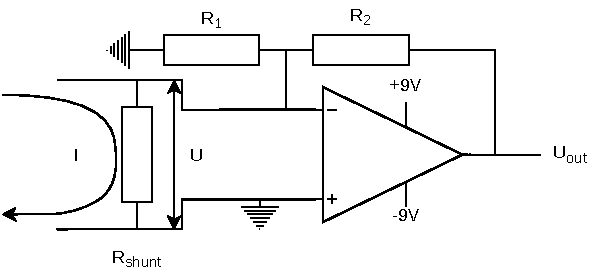
\includegraphics[width=.4\textwidth]{../../../Figures/shuntamp_sketch/shuntamp.pdf}
	\caption{Current measurement circuit using an operational amplifier and a shunt resistor.}
	\label{fig:shuntamp}
\end{figure}
Using Ohm's law and the golden rules of operational amplifiers, see section \ref{sec:theory:amplifiers}, the simple relation in equation \ref{eq:shuntamp} can be derived.
\begin{align}
	U_\text{out} & = R_\text{S}I\label{eq:shuntamp}
\end{align}
This first amplification stage uses an AD549LHZ \ac{opamp} which features a high input impedance, low input current and offset voltage adjustment \cite{AD549}. According to its datasheet, it is designed to be used for electrometer amplifiers or photodiode interfaces. Driving the amplifier with a bipolar supply allows measurement of both positive and negative currents. For matching the bipolar voltage signal from the input stage with the unipolar \ac{adc} input, a second amplifier is introduced as depicted in figure \ref{fig:frontendsketch}, expanding equation \ref{eq:shuntamp} to:
\begin{align}
	U_\text{ADC}=IR_\text{S}+U_\text{ref}
	\label{eq:frontend:old:transferfunction1}
\end{align}
Where $U_\text{ref}=\SI{2.048}{\volt}$.
\begin{figure}
	\centering
	\includegraphics[width=.8\textwidth]{../../../Figures/shuntamp_sketch/frontendsketch.pdf}
	\caption{Front-end circuitry used in the revisions 3 and 4. The additional \ac{ovp} diodes are depicted in figure \ref{fig:frontend:old:ovp2}.}
	\label{fig:frontendsketch}
\end{figure}
As a second amplifier, the $\mu$A741 is used. It is a general-purpose amplifier, designed for voltage amplification.
For digitisation, the design uses the AD7790 buffered $\Sigma\Delta$ \ac{adc} which features a suitable low noise for the application and has a sampling frequency of \SI{9.5}{} to \SI{120}{\hertz} \cite{AD7790}. Taking into account the digitisation range of the \ac{adc} and the highest shunt resistance of \SI{100}{\mega\ohm} the setup could reach a theoretical precision of \SI{0.625}{\pico\ampere}. 

\subsection*{Over-Voltage Protection}
\label{sec:status:ovp}
The \acp{pAM} are equipped with protection diodes as depicted in figure \ref{fig:frontend:old:ovp1}, to prevent damage to the amplifier from over-voltage conditions. In figure \ref{fig:frontend:old:ovp2} an extension to the input stage is depicted, which is soldered floating over the board. It consists of a \SI{20}{\kilo\ohm} resistor in parallel to a SA5.0CA bipolar TVS diode\footnote{It is unknown why this circuitry was attached or by whom. It was already mentioned in \cite{bugl} in 2013.}. The resistor forms a voltage divider with the \SI{5}{\kilo\ohm} resistor, adding an extra factor to the transfer function. The transfer-function in equation \ref{eq:frontend:old:transferfunction1} is expanded to:
\begin{align}
U_\text{ADC}=1.25\cdot IR_\text{S}+U_\text{ref}
\label{eq:frontend:old:transferfunction2}
\end{align}
The influence of the TVS diode will be discussed in section \ref{sec:nonlinearity}.
\begin{figure}
	\begin{subfigure}{\textwidth}
		\centering
		\includegraphics[width=0.8\textwidth]{../../../Figures/shuntamp_sketch/frontendsketchwOVP1.pdf}
		\caption{Front-end equipped with over voltage protection diodes between the inputs of the first amplifier.}
		\label{fig:frontend:old:ovp1}
	\end{subfigure}\hfill
	\begin{subfigure}{\textwidth}
		\centering
		\includegraphics[width=0.8\textwidth]{../../../Figures/shuntamp_sketch/frontendsketchwOVP2.pdf}
		\caption{The same front-end with additional \SI{20}{\kilo\ohm} resistor and parallel SA5.0CA TVS-diode.}
		\label{fig:frontend:old:ovp2}
	\end{subfigure}
	\caption{The two expansions that are made to the front-end depicted in figure \ref{fig:frontendsketch}.}
\end{figure}
\subsection*{Selectable Modes}
As introduced before the \acp{pAM} have a selectable resolution and measurement range. This is achieved by adding a second smaller resistor $R_\text{||}$ in parallel to the \SI{100}{\mega\ohm} resistor; this reduces the shunt resistance to:
\begin{align}
	R_\text{S}=\frac{1}{\frac{1}{R_{||}}+\frac{1}{\SI{100}{\mega\ohm}}}
\end{align} 
Modes for the different revisions are shown in table \ref{tab:frontend:old:modes}. The low-resolution modes also use a varistor parallel to the shunt resistor as additional over-voltage protection.
\begin{table}
	\centering
	\begin{tabular}{cccccc}
		\hline
		mode & shunt resistance & range & resolution & \multicolumn{2}{c}{raw mode} \\
		 & 						 & & 		& revision 3 & revision 4 \\
		\hline
		1 & \SI{100}{\ohm}$||$\SI{100}{\mega\ohm} & \SI{\pm16.4}{\milli\ampere} & \SI{625}{\nano\ampere} & 0 & \\
		2 & \SI{10}{\kilo\ohm}$||$\SI{100}{\mega\ohm} & \SI{\pm164}{\micro\ampere} & \SI{6.25}{\nano\ampere} & 1 & 0 \\
		3 & \SI{100}{\kilo\ohm}$||$\SI{100}{\mega\ohm} & \SI{\pm16.4}{\micro\ampere} & \SI{625}{\pico\ampere} & & 1 \\
		4 & \SI{1}{\mega\ohm}$||$\SI{100}{\mega\ohm} & \SI{\pm1.64}{\micro\ampere} & \SI{6.25}{\pico\ampere} & 2 & 2 \\
		5 & \SI{10}{\mega\ohm}$||$\SI{100}{\mega\ohm} & \SI{\pm164}{\nano\ampere} & \SI{0.625}{\pico\ampere} & & 3 \\
		6 & \SI{100}{\mega\ohm} & \SI{\pm16.4}{\nano\ampere} & \SI{0.5}{\pico\ampere} & 3 & 4 \\
		\hline
	\end{tabular}
	\captionof{table}{Modes of the different \ac{pAM}, the range is given by $\frac{\text{\SI{2.048}{\volt}}}{1.25\text{R}_\text{S}}$. This sets the resolution to range divided by $2^{15}$. Translated and modified from \cite{rudolph}.}
	\label{tab:frontend:old:modes}
\end{table}
\section{High-Voltage Isolation}
The \acp{pAM} are designed for usage on the high-voltage supply lines of a \ac{gem}-foil. This requires some precautions to protect a user. To ensure isolation, the \acp{pAM} are enclosed in a plastic box. The only openings in this box are the terminals for the signal lines. The terminals are SHV connectors, the outer conductor is connected to earth ground, only the inner conductor is on a high-voltage. \\
As a power supply the devices use \SI{9}{\volt}-blocks, as these allow operation without any ground connection. In addition, a photovoltaic powering was developed, to achieve longer run times, see \cite{rudolph} for details.
\section{Design Performance}
\subsection{Power Consumption}
The power consumption characteristics were studied by \cite{rudolph} and are only briefly summarized here. Originally the devices are powered by \SI{9}{\volt}-block batteries, hence low power consumption is a design goal. Table \ref{tab:frontend:old:power} summarizes the current draw for an operating device.
\begin{table}
	\centering
	\begin{tabular}{lr}
		\hline
		Average & current draw \SI[per-mode=symbol]{}{\per\milli\amp}\\ \hline
		without XBee & \SI{1.773\pm0.012}{} \\
		with the Xbee sending & \SI{48.1\pm0.6}{} \\
		\hline
	\end{tabular}
	\captionof{table}{Current draw of a \ac{pAM}. From \cite{rudolph}, modified.}
	\label{tab:frontend:old:power}
\end{table}
\subsection{Measurement Results}
The measurement performance of the device was analysed by \cite{roedel}. It was found that the devices show a characteristic non-linear behaviour with deviations in the range of some ten \ac{pA} in the most sensitive mode. This non-linearity scales linear with temperature, which was also shown by \cite{roedel}. The origin of the effect is discussed in section \ref{sec:nonlinearity}.

Calibration measurements showed that the error on the \ac{pAM} reading, the standard deviation of 128 measurements, is around 1.5 to 2 \ac{adc} channels, resulting in an uncertainty of around \SI{1}{\pico\amp}. Showing that the design is capable of precise measurements on the \ac{pA} scale.

The \ac{pAM} take \SI{8}{\second} to finish a complete sample of 128 \ac{adc} readings. This is mainly due to the low \ac{adc} sampling rate that is used. This low sample rate results in a bad time resolution.

\section{Infrastructure}
To operate the \ac{pAM} the firmware for the \ac{uC} is needed, as well as the \ac{pamos} software; which is responsible for receiving the data, applying the calibration and saving the results. To obtain a reliable calibration for the \acp{pAM}, a calibration station was built by \cite{roedel}. A short introduction to the software is given here.
\subsection{Firmware}
\label{sec:firmwareold}
With the beginning of this thesis, the \ac{msp} firmware is present in versions 3 and 4 for the respective revisions of the design. It is written in C and compiled via the opensource msp430-gcc compiler in version 3.2.3; which is only running on Ubuntu 10.04.4 LTS, according to \cite{agwiki}. The rather complicated flashing process is described there as well. 
The basic workflow of the firmware is depicted in figure \ref{fig:firmware:old:workflow}.\\
\begin{figure}
	\centering
	\includegraphics[width=.8\textwidth]{../../../Figures/pAMworkflow/old/mainloop/main.pdf}
	\caption{\ac{pAM} firmware workflow for firmware versions 3.x.}
	\label{fig:firmware:old:workflow}
\end{figure}
The firmware comes in different builds featuring different functionalities. The firmware versions x.0 are the basic versions, the versions x.1 additionally send out all 128 \ac{adc} raw values. All firmware versions also have a second build, that sets the \textit{CALIB} flag, which adds auto mode switching to the firmware.

To simplify coding and increase readability of the code, a lot of alternative symbols are defined in the header files \textit{iostructures.h} and \textit{pAM-definitions.h}. 
The ports and pins were assigned an alias according to their purpose. For example, the \ac{adc} communication is done with port 3, pins 0 to 3, hence the aliases are:
\begin{lstlisting}[style=cpp]
#define ADC_PORT port3
#define ADC_SCLK pin3 /* P3.3 SCLK */
#define ADC_DOUT pin2 /* P3.2 SOMI */
#define ADC_DIN pin1 /* P3.1 SIMO */
#define ADC_CNV pin0 /* P3.0 */
\end{lstlisting}


\subsubsection*{Initilisation}
On start-up of the microcontroller, some basic settings have to be made. At first, the clock and timer modules have to be set up. The device is equipped with a \SI{32}{\kilo\hertz} crystal on \pin{XIN} and a \SI{1.8}{\mega\hertz} crystal on \pin{XT2}. As main clock source in the \acp{pAM}, the \SI{1.8}{\mega\hertz} clock is used.

The next step is to set up the pins according to their purpose. Each port has several registers defining their usage, see table \ref{tab:firmware:portregisters}. This happens with the function \code{port\_setup()}, the registers for the different ports are summarized in table \ref{tab:firmware:portregisters}.
\begin{table}
	\centering
	\begin{tabular}{clccccc}
		\hline
		register & register purpose &\multicolumn{3}{c}{ports}&\multicolumn{2}{c}{states} \\
		 & & 1 & 2 & 3 - 6 & 1 & 0 \\\hline 
		dir & select if pin is input or output &\checkmark&\checkmark&\checkmark& output & input \\
		in & state applied to pin &\checkmark&\checkmark&\checkmark& \multicolumn{2}{c}{set externally}\\
		out & state applied to pin &\checkmark&\checkmark&\checkmark& set output high & set output low \\
		sel & function selection &\checkmark&\checkmark&\checkmark& peripheral module & I/O functionality\\
		ie & interrupt enable &\checkmark&\checkmark& & interrupt enabled & interrupt disabled\\
		ies & interrupt edge select &\checkmark&\checkmark&& falling edge & rising edge\\
		ifg & interrupt flag &\checkmark&\checkmark&& interrupt pending & no interrupt pending \\
		\hline
	\end{tabular}
	\captionof{table}{Registers, their purpose and ports that feature them. Only ports 1 and 2 have interrupt capability \cite{msp_manual}.}
	\label{tab:firmware:portregisters}
\end{table}
The USART module is set up to interface the \acs{xbee}, as depicted in listing \ref{lst:firmware:old:usart}. The modules setup allows two-way communication. However, the communication protocols for this are not implemented.
\begin{codecpp}[caption={Setup of the USART ports for communication with the \acs{xbee} \label{lst:firmware:old:usart}. Comments preceded with \textit{//<} were added for explanation.}]
void usart_setup() {
	/*TX*/
	//<TX pin for transmitting data: 
	port3.dir.pin4 = IO_DIRPIN_OUTPUT; //<=1
	port3.sel.pin4 = IO_ALTPIN_SELECT;//<=1
	/*RX*/
	//<RX pin for receiving data:
	port3.dir.pin5 = IO_DIRPIN_INPUT; //<=0
	port3.sel.pin5 = IO_ALTPIN_SELECT;//<=1
	
	ME1 |= UTXE0 + URXE0; // USART0 TX, RX enable
	//<set protocol to 8 data-bits, 1 stop-bit, no parity (8N1):
	U0CTL |= CHAR;		 // 8 data-bits, 1 stop-bit, no parity (8N1)
	//< set clock source to MCLK (1.8MHz): 
	U0TCTL |= SSEL_2;	 // UCLK <- SMCLK	
	/* clock: 1843200Hz
	desired baud rate: 115200bps
	division factor: 16
	effective baud rate: 115200bps
	maximum error: 0us 0.00%
	*/	
	//< set divider to 16, 	modulation to 0:
	U0BR0=0x10; U0BR1=0x00;	U0MCTL=0x00;
	//<open USART for operation:
	U0CTL &= ~SWRST;			/*USART freigeben*/
}
\end{codecpp}
After these setups, the mainloop is started. First the \ac{adc} is reset, and the LED blinks to signal operation. After this the \ac{adc} is setup for reading data. The firmware reads 128 values from the \ac{adc}, entering a low power mode in between conversions. The \ac{adc} \pin{RDY} pin is used as an interrupt to enter the corresponding \ac{ISR}, which handles data reading.

After data is read-out, mean and standard deviation of the 128 values is calculated. This averaging has the advantage of reducing the influence of noise on the data and allows more precise measurements. However, it elongates the readout time. The derived values get sent out along with other parameters. The data frame for the firmware revisions x.0 is depicted in figure \ref{fig:firmware:vx0:dataframe}; the versions x.1 packages are shown in figure \ref{fig:firmware:vx1:dataframe}. Afterwards, the readout is finished, and another cycle starts.
\begin{figure}
	\centering
	\begin{tabular}{|C{4cm}|C{4cm}|C{1cm}|C{1cm}|C{1cm}}
		\cline{1-4}
		mean & error & mode & voltage & \dots \\
		\cline{1-4}
		\multicolumn{5}{c}{}
		%\mc{4 byte} & \mc{4 byte} & \mc{1 byte} & \mc{1 byte} \\ 
	\end{tabular}
	\begin{tabular}{C{1cm}|C{4cm}|C{4cm}|C{1cm}|}
		\cline{2-4}
		\dots & conversion time & time until sending & 0\\
		\cline{2-4}
		\multicolumn{4}{c}{}
		%\multicolumn{}{c}{}
		%\mc{4 byte} & \mc{4 byte} & \mc{1 byte} & \mc{1 byte} \\ 
	\end{tabular}
	\captionof{figure}{Datasets as sent out by \acp{pAM} running the firmware v3.0 and v4.0. The package contains mean and error of the acquired data, the current operating mode, the SVS voltage output, the time needed for conversion, the time between finishing a conversion and sending data, and the number of remaining packages; which is 0 in this case.}
	\label{fig:firmware:vx0:dataframe}
\end{figure} 
\begin{figure}
	\centering
	\begin{tabular}{|C{4cm}|C{4cm}|C{1cm}|C{1cm}|C{1cm}}
		\cline{1-4}
		mean & error & mode & voltage & \dots \\
		\cline{1-4}
		\multicolumn{5}{c}{}
		%\mc{4 byte} & \mc{4 byte} & \mc{1 byte} & \mc{1 byte} \\ 
	\end{tabular}
	\begin{tabular}{C{1cm}|C{4cm}|C{4cm}|C{1cm}|}
	\cline{2-4}
	\dots & conversion time & time until sending & 4\\
	\cline{2-4}
	\multicolumn{4}{c}{}
	%\multicolumn{}{c}{}
	%\mc{4 byte} & \mc{4 byte} & \mc{1 byte} & \mc{1 byte} \\ 
	\end{tabular}
	\begin{tabular}{|C{2cm}|C{2cm}|C{3cm}|C{2cm}|C{1cm}|}
	\cline{1-5}	%\cline{4-5}
	\ac{adc} value & \ac{adc} value & \dots &\ac{adc} value & 3\\
	\cline{1-5}	%\cline{4-5}
	\ac{adc} value & \ac{adc} value & \dots &\ac{adc} value & 2\\
	\cline{1-5}	%\cline{4-5}
	\ac{adc} value & \ac{adc} value & \dots &\ac{adc} value & 1\\
	\cline{1-5}	%\cline{4-5}
	\ac{adc} value & \ac{adc} value & \dots &\ac{adc} value & 0\\
	\cline{1-5}	%\cline{4-5}
	%\mc{4 byte} & \mc{4 byte} & \mc{1 byte} & \mc{1 byte} \\ 
	\end{tabular}
	\captionof{figure}{Datasets as sent out by \ac{pAM} running the firmware v3.1 and v4.1. The first package contains mean and error of the acquired data, the current operating mode, the SVS voltage output, the time needed for conversion, the time between finishing a conversion and sending data, and the number remaining packages. The next four packages contain 32 \ac{adc} readings each, followed by the number of remaining packages.}
	\label{fig:firmware:vx1:dataframe}
\end{figure} 

\subsection{\acs{pamos}}
The \acl{pamos} is the software used to receive and handle data, send out by the \acp{pAM}. It is written in \acs{cpp} to be run on Linux machines. With the beginning of this work, it was available in version 2. The software reads data, applies the calibration and stores data in an online database or locally as a root file. Discrimination between the firmware versions described above is done by the message length. 

\subsection{CalibAna}
The CalibAna software was developed by \cite{roedel}. A detailed description of its principle can be found there. It controls the calibration setup by communicating with, an Arduino to adjust the temperature, the \ac{keithley}, which used as a reference for calibration and reads the \ac{pAM} data. The output can be stored in a calibration database and be used to create a plot with the calibration data, using a gnuplot script. An example plot is shown on figure \ref{fig:CalibAna2:example}. The top left plot shows current measured by the Keithley vs \ac{adc} readings and a linear fit of the data. The central plot contains the deviation of current values from the linear fit applied to the \ac{adc} channel range. These deviations are fitted with a third-order polynomial. The bottom left plot shows the deviations from the polynomial fit as a histogram. A gaussian fitted to the histogram is used to approximate the resolution of the \ac{pAM}. 
\begin{figure}
	\centering
	\includegraphics[width=\textwidth]{../../../Figures/pAMOld/Measurements/cal_stat16_rmode0_rand_temp_2017-01-18_00.34_plot.pdf}
	\caption{Calibration plot produced by CalibAna2.}
	\label{fig:CalibAna2:example}
\end{figure}


\section{Motivation}
Now, having provided a look into the device, why is a revision of the design necessary?
There are several shortcomings in operation and handling of the design that were discovered over time. 
As described above, the firmware is not up to date and is not compatible with modern compilers. Hence upgrading the firmware is one of the bullet points.
This process can also be used to add new features to the firmware to make operation of the device more flexible.

A problem that occurs during operation is a breakdown of the \ac{opamp} in the input stage, probably due to over-voltage conditions on the inputs. On the one hand, replacement of an amplifier is complex and rather costly with $\approx$\SI{60}{\euro} per amplifier.  On the other hand, the running measurement is interrupted and needs to be repeated. \\
One of the biggest issues, in the end, is non-linear current to \ac{adc} channels relation mentioned above in combination with a temperature dependence, making a complex and time-consuming calibration necessary.
%It was desired to have the ability to see the measurement result in real time over a display, this was addressed by \cite{bugl}, but lead to a more noisy measurement in operation.









% !TEX root = mythesis.tex
% !TeX spellcheck = en_GB
%==============================================================================
\chapter{Addressing the Issues}
\label{sec:problem_solving}
%==============================================================================
In chapter \ref{sec:current_status} an introduction on open topics was given. An update of the firmware, investigations on the cause of the non-linear behaviour and development of a new \ac{ovp} solution are necessary. These three topics will be addressed in this chapter.

\section{Firmware Update}
\label{sec:newfirmware}
As previously stated, the firmware for the \ac{pAM} is not compatible with the compiler provided and maintained by \ac{TI}. One of the goals in the scope of this work was to adapt the firmware to achieve compatibility. As this progress requires some significant changes in the code, it was used to develop new features and restructure the program, in parallel.
\subsection{Code Syntax}
To be compatible with the compilers provided by TI some changes to the syntax of the code were necessary.
\subsubsection*{Pin addressing}
One of the biggest changes that had to be made was the way the pins and ports of the \ac{uC} were addressed. In the previous firmware versions, the pins and ports were accessible similarly to objects, via the "." operator. The new compiler fills registers from 8-bit numbers. As an example, the direction of pin 2 of port 1 should be set to 1, allowing usage as an output pin.On the Left, the way it was done with the previous compiler; On the right, the way the new compiler requires:\\
\begin{minipage}{\textwidth}
\begin{minipage}{0.49\textwidth}
\begin{lstlisting}[style=cpp]
port1.dir.pin2 = 1;
\end{lstlisting}
\end{minipage} 
%\hfill\vrule\hfill
\begin{minipage}{0.49\textwidth}
\begin{lstlisting}[style=cpp]
port1_dir = 0b00000100;
\end{lstlisting}
\end{minipage}
%\centering
%\captionof{lstlisting}{How to set the direction of port 1, pin 2 to serve as output. On the left, the program accesses pin2 in the dir register of port2. On the right, the value of the register port1\_dir is set.}
%\label{code:compare1}
\end{minipage}\\
\newline
Register content can be changed in two ways. Either assigning a value to the register, however, this would overwrite the status of all other pins. This can be circumvented by using a-bitwise operation:
\begin{lstlisting}[style=cpp]
port1_dir |= 0b00000100;
\end{lstlisting}
The 8-bits are individually or' ed with the 8-bits of $0b00000100$, changing the value of the second-bit without influencing the other-bits.
The inverse operation to this is-bitwise \textit{not and}:
\begin{lstlisting}[style=cpp]
port1_dir &=~ 0b00000100;
\end{lstlisting}
To further increase readability, the-bitwise operations were assigned aliases. A small example:
\begin{lstlisting}[style=cpp]
#define set_high |= 
#define set_low &= ~
\end{lstlisting}
Correspondingly the binary numbers that represent each pin are assigned with the pin name:
\begin{lstlisting}[style=cpp]
#define pin0 0b00000000
#define pin1 0b00000010
\end{lstlisting}
The initial example hence is now written as:
\begin{lstlisting}[style=cpp]
port1_dir set_high pin2;
\end{lstlisting}

%\subsubsection*{Interrupt routine}
%Another change in syntax was the declarations of interrupt routines

\subsection{File Structure}
To ease handling of the code, it was split up in different source files and their headers. All functions concerning the \acs{xbee} for example, are gathered in \textit{xbee.c} with the corresponding \textit{xbee.h}. These files are shared between the different versions of the firmware, allowing introduction of new features on all of them.

\subsection{Bidirectional Communication}\label{sec:2waycom}
As mentioned before there, are possible options that change behaviour and output of the \ac{pAM}. The options are set together with the receiver address in the flashing process. The devices can be made more flexible by allowing wireless two-way communication between a \ac{pAM} and the receiving computer. The hardware setup of all generations of \acp{pAM} already supports this. On the software side, functions handling the reception of data are needed. 
The parameters need to be set before the measurement is started. Therefore, the firmware was modified to enter an idle state on start-up, waiting for a handshake with the external setup. To indicate the device is waiting for setup, the indicator LED is turned on. The \code{set\_up} flag is introduced to indicate that the device has been set up successfully. 
As the USART module of the MSP430 has interrupt capability, the corresponding \ac{ISR} will be used to handle incoming messages. 

An \acs{xbee} module will immediately send out data it received in an \ac{api} frame, see section \ref{sec:theory:XBee}. The \ac{uC} will read the first character, store it in the \ac{USART} receive buffer (U0RXBUF) and set the \ac{USART} receive interrupt flag (URXIFG0). This generates an interrupt request, causing the program to jump to the \ac{USART} interrupt routine. 

The \ac{ISR} at first checks if the device is already setup. Next step is to disable the \ac{USART} interrupt and hold the Watchdog timer. The received data is read using the \code{rx\_request()} function. 
This function will read the message characters into a buffer array by polling on URXIFG0. To simplify the message handling on the microcontroller site, an upper limit \code{length} was set on the message length, and the char \code{0xFF} was reserved to indicate the end of the message. The polling is stopped when either \code{length} bytes were read or the second to last byte was the end of message indicator.
From the message array, the parameters are derived by scanning for two indicators. The first indicates that the next two bytes contain the address of the receiving station. The second indicates that the following bytes contain the runtime parameters. Currently, there are two parameters for the revisions three and four to be set. The sensitivity mode to operate in and if the \ac{adc} raw values are to be sent in addition.
The list of parameters can be extended in the future.\\


To ensure correct setup, the \ac{pAM} answers with a frame containing all the set flags. The USART interrupt is disabled after this handshake, to ensure stable operation.
It was tried to allow changing the parameters during runtime by allowing further interrupts. This led to spurious interrupts, disturbing the device operation. 

A flow-diagram showing this initialisation loop can be found in figure \ref{fig:firmware:new:init}.
\begin{figure}
	\centering	\includegraphics[width=.8\textwidth]{../../../Figures/pAMworkflow/new/initialization/initilization.pdf}
	\caption{The initialisation process for \ac{pAM}, as implemented in the firmware versions 3.2 and 5.0.}
	\label{fig:firmware:new:init}
\end{figure}

Only after this handshake of the \ac{pAM} with the external setup, readout is possible, as introduced in section \ref{sec:firmwareold}.

The changes described above are combined in the firmware version 3.2.
To ensure compatibility with the new firmware, the \ac{pamos} and \ac{calibana} software were modified. The necessary modifications are discussed in the next section.

\subsection{Changes to PAMOS}
The \ac{pamos} software is handling the data acquisition of the \ac{pAM} on the computer side. It is the main software used to communicate with the devices. It needs to be adapted to support the two-way communication implemented in the firmware. A first approach was to use one of the various open-source libraries available for the XBee modules. The \textit{libxbee3} library \cite{libxbee} was chosen. The approach was discarded after the library proved to be to slow to keep up with the revision 5 of the \ac{pAM}, developed in chapter \ref{sec:newfrontend}. 

Therefore, a custom solution was developed based on the \textit{termios} library \cite{termios}, which was already used for data reading in the previous version of \ac{pamos}. The \textit{termios} library provides a set of functions that can be used to control an asynchronous communication port of a computer, e.g. the USB port. Reading and writing to the port is handled as it is done for regular files. The message handling on the computer side was made more complex, including different error-handling methods. This is possible, as a computer is noticeably faster than the \ac{msp} used in the \acp{pAM}.

An introduction on the functions created around this library to manage the \ac{pAM} communication will be given here. To ease handling, all \ac{pAM} related variables and functions are gathered in the \code{pAMeter} class:
\begin{codecpp}[caption={pAMeter structure in the \ac{pamos} software. The structure contains all parameters that are necessary to allow flawless communication.}]
class pAMeter {
	public:
	int fd; //!< file descriptor pointing to a file managed by a termios structure. Used to read and write from usb port
	unsigned int station; //!< The stations 16-bit address, filled from startup argument -s
	unsigned int receiver; //!< The 16-bit address of the receiver used, filled from startup argument -r
	unsigned char mode; //!< The mode the pAMeter should use, filled from startup argument -m
	unsigned char dataFormat; //!< Determines what data to be transmitted, filled from startup argument -F
	unsigned char REVISION; /*!< Revision of the pAMeter in use, transmitted by the pAM on setup. Can be mapped to a readable value with calc_mode()*/
	unsigned int frame_id = 0; //!< frame id for counting frames
	unsigned char delay; //!< Rev 5 only, determines the number of wait cycles put between two readings
	int debug=1;
	struct pAMmessage msg; //!< used to store a single frame transmitted by a pAMeter
	std::map<unsigned short, int> revision; //!
	std::map<unsigned short, calibration_t> cal; //! contains the calibration for the station
	int initiate(); //!< organizes the setup of a pAM with mode, dataFormat etc. and checks if the setup was successfull
	int setup_interface(); //!< sets up all termios attributes and applies them to the file behind fd
	int send_init(); //!< sends the initialisation frame and checks for a confirm
	int TX(unsigned char buffer, unsigned int length); //!< transmits buffer with size length with the defined api framework
	int RX(); //!< used to receive a frame and store it in a pAMmessage, verifies checksum
	std::tuple<unsigned char, unsigned int> message_handler(); //!< identifies a received message and fills the pAMmessage 	
};
\end{codecpp}
\subsubsection{Initialisation}
The port is handled alike a file, as stated before. Therefore, the first step is to open the port and link it to the file descriptor \textit{fd}:
\begin{lstlisting}[style=cpp]
pAM->fd = open("/dev/ttyUSB0", O_RDWR | O_NOCTTY);
\end{lstlisting}
The \textit{termios} library associates a terminal to the file that handles the communication. This terminal has to be set up with the communication parameters, e.g. baud rate, parity, word length. This is done by the \code{setup\_interface()} function. This allows flawless communication with the \acs{xbee}. The initialisation of the \ac{pAM} is done in the \code{initiate()} function.
The first step is to send out the initialisation frame for the \ac{pAM}, see section \ref{sec:2waycom}. This is done by the \textit{TX()} function, shown in listing \ref{lst:pamos:TX}. It fills all required frame data in the \code{buffer} array and calculates the checksum.
Afterwards, the array is written to the USB port, but it is only transmitted if the data is followed by the carriage return character \code{"\textbackslash r"}. The sending is repeated until an acknowledge from the XBee is received. If a frame is received, that is no acknowledge, the program prints an error message and holds, as a successful setup can not be guaranteed.
When an acknowledge is received, the program awaits the confirmation frame from the \ac{pAM}. If one of the parameters in the confirmation frame does not match, the program returns an error message and stops.
\begin{codecpp}[caption={\ac{cpp} function for transmitting data with an XBee module and checking if an acknowledge was received\label{lst:pamos:TX}.}]
int pAMeter:: TX(unsigned char* buf, unsigned int length)
{
	tuple<unsigned char, unsigned int> handle;
	unsigned char buffer[1 + 2 + 1 + 1 + 2 + 1 + length + 1];
	buffer[0] = 0x7e;
	buffer[1] = ((length + 5) >> 8);
	buffer[2] = ((length + 5) & 0x00ff);
	buffer[3] = 0x01;
	buffer[4] = 1; //frame_id++;
	buffer[5] = (station >> 8);
	buffer[6] = (station & 0x00ff); 
	buffer[7] = 0x00;
	for (unsigned int i = 0; i < length; i++) {
		buffer[i + 8] = buf[i];
	}
	buffer[8 + length] = 0;
	buffer[8 + length] = checksum(buffer, sizeof(buffer));
	do {//< send until acknowledge is received
		sleep(0.3);
		write(fd, buffer, sizeof(buffer));
		write(fd, "\r", sizeof("\r"));
		sleep(0.5);
		if (RX() == 1) {
			handle = message_handler();//< analyzes the received frame
			if ((get<0>(handle) == 0x89) && (get<1>(handle) == 0)) {
				//< is acknowledge
				if(debug) cout << "send init success" << endl;
				return 1;
			} else {
				printerr("TX failed", " ");
				return 0;
			}
		}
	} while (1);
	return 1;
}
\end{codecpp}
\subsubsection{Receiving Data}
The \code{RX()} function, see listing \ref{lst:pamos:RX}, reads one char from the port. If the char is the frame delimiter from an XBee \ac{api} frame, the function will try to read the message, else it will return a \textit{nothing received}. 
The next two chars in the buffer should be message length, see section \ref{sec:theory:XBee}. The message length is extracted from these, and a message of this length is read. The message is validated by calculating its checksum. If the checksum does not hold, \textit{invalid message} is returned. The full message is stored in the message buffer to be further analysed by the \code{message\_handler()} function.
\begin{codecpp}[caption={\ac{cpp} function, that reads data from the USB port\label{lst:pamos:RX}.}]
int pAMeter::RX()
{
	unsigned char del = 0;
	read(fd, &del, 1);
	if (del == 0x7e) {
		char len_buf[2] = { 0 };
		read(fd, &len_buf, 2);
		msg.length = ((len_buf[0] << 8) + (len_buf[1]));
		if(debug) cout << "received massge w length : " << msg.length << endl;
		if ((msg.length < 0) | (msg.length > 255)) {
			printerr("message length out of boundaries");
			cout << msg.length << endl;
			return 0;
		}
		read(fd, &msg.buffer, msg.length);
		unsigned char checksum_buf[1];
		read(fd, &checksum_buf, 1);
		msg.checksum = checksum_buf[0];
		unsigned char temp = 0;
		for (unsigned int i = 0; i < msg.length; i++) {
			if(debug)cout << " " << (int)msg.buffer[i];
			temp += msg.buffer[i];
		}
		if(debug)cout << endl;
		if (msg.checksum + temp != 255) {
			printerr("checksum not valid");
			return 0;
		}
		return 1;
	} else {
		if(debug)cout << "not received anything" << endl;
		return -1;
	}
}
\end{codecpp}
The \code{message\_handler()} function identifies the type of \ac{api} frame and extracts the contained data.


\subsection{Changes to CalibAna}
\label{sec:solving:calibana}
For the CalibAna software, similar functions were implemented to control the \ac{pAM}. However, the increased readout frequency of the new revision, developed in chapter \ref{sec:newfrontend}, caused problems.
The Keithley, needs some time to perform a precise measurement\footnote{The influence of measurement time on the precision is briefly discussed in section \ref{sec:results}}. To ensure this, the data acquisition is artificially lengthened by adding a delay of one second. The fast \ac{pAM} will perform multiple measurements during this time, leading to a pile-up.
Reading from the port read the next available message, not the last received one. A single read command per voltage step hence will result in outdated data. To work around this problem, the reading process was moved to a separate thread running the \code{continousread()} function, see listing \ref{lst:calibana:contread}. The function calls \code{RX()} until a frame is received. The \code{message\_handler()} function checks if the received message is a receive frame, which sets the \code{valid} flag. When the most recent frame is to be saved for calibration, the main program sets the \code{pause} flag, holding the readout when the next valid data-frame is available.
\begin{codecpp}[caption={\ac{cpp} function, that continuously tries to read from the USB port and on success stores the message\label{lst:calibana:contread}.}]
void pameterneu::continousread()
{
	while (!stop) {
		valid = 0;
		tuple<unsigned char, unsigned int> handle;
		sleep(0.2);
		int status;
		do {
			status = RX();
		} while (!(status==1));
		handle = message_handler();
		if (!((get<0>(handle) == 0x81) && (get<1>(handle) == 1))) {
			valid = 0;
		} else {
			valid = 1;
		}
		while (valid && pause) {
			cout << "waiting for data read" << endl;
		}
	}
}
\end{codecpp}
\subsubsection*{CalibAna Data Analysis}
To simplify data analysis and allow more flexibility, a new plot program was developed using \textit{python}, to replace the gnuplot script developed by \cite{roedel}. Python was chosen as it is more versatile than gnuplot and more commonly known. %\footnote{And due to the authors lack of knowledge about gnuplot.}
The plot program was developed to be capable of producing calibration data for the revision 3 and 4 \ac{pAM} as well as the revision 5 devices.
The calibration data output of CalibAna was modified, adding a header to the file. The header contains calibration parameters like mode, number of measurement runs, station and revision. The python script reads data from this header and uses it to fit calibration functions to the data and produce plots according to the revision and range.


\section{Non-Linear Measurements}
\label{sec:nonlinearity}
As introduced above the devices show a characteristic non-linearity; the origin of this is explored here. 
The non-linearity can be found on all modes of sensitivity, see figure \ref{fig:measurement:old:comparemodes}. Hence the effect seems to be independent of the measured current and probably occurs in the voltage signal shaping of the front-end.
\begin{figure}
	\centering
	\begin{subfigure}{\textwidth}
		\includegraphics[width=\textwidth,page=1]{../../../Figures/pAMOld/Measurements/cal_stat16_rmode0_rand_temp_2017-01-18_00.34_plot.pdf}
	\end{subfigure}
	\begin{subfigure}{\textwidth}
	\includegraphics[width=\textwidth,page=1]{../../../Figures/pAMOld/Measurements/cal_stat16_rmode3_rand_temp_2017-01-16_10.33_plot.pdf}
	\end{subfigure}
	\caption{Calibration measurement for station 16 in lowest and highest sensitivity mode.}
	\label{fig:measurement:old:comparemodes}
\end{figure}
For investigation, the front-end was simulated using LTspice. The effect could not be reproduced quantitatively, as a model for the SA5.0CA Diode was missing. However using a model for a diode of a similar type, it could be shown, that the diode adds a non-linear characteristic to the design. The non-linearity is caused by the diode clipping the feedback voltage, which propagates to the output voltage.
Measurements, done with all diodes removed, indeed showed no such effects, see figure \ref{fig:measurement:old:noOVP}.
\begin{figure}
	\centering
	\includegraphics[width=\textwidth,page=1]{../../../Figures/example_pAmeter_old/old_no_ovp.pdf}
	\caption{Calibration measurement for a station with removed diodes.}
	\label{fig:measurement:old:noOVP}
\end{figure}
Removing diodes from the front-end leaves the \ac{pAM} without over-voltage protection. A new solution has to be found; the next sections will treat this topic.
 
\section{Over-Voltage Protection}
\label{sec:solving:ovp}
The \acp{pAM} are operated at high voltages. Fast ramping or higher than expected currents, e.g. discharges in the \acp{gem} attached, can lead to large voltage differences between the input terminals. Such over-voltage conditions can result in malfunction of the input stage amplifier. To prevent such events, diode clamping is a commonly used technique. As introduced in section \ref{sec:status:ovp}, the devices come with two \ac{ovp} structures. 
The first one consists of two antiparallel diodes between the \ac{opamp} inputs, see figure \ref{fig:frontend:old:ovp1}. These diodes are no appropriate \ac{ovp}, as they connect the non-inverting amplifier input, with the inverting input. As introduced in section \ref{sec:theory:amplifiers}, an ideal \ac{opamp} adjusts the output to have matching inputs. Applying large differential voltages between the inputs can lead to the destruction of an amplifier. In this setup, however, the inverting input is only defined by the output voltage and the feedback loop. An over-voltage condition between the \ac{opamp} inputs is highly improbable. 

A similar argument is valid for the SA5.0CA diode that was added to the feedback loop, see figure \ref{fig:frontend:old:ovp2}. It limits the feedback loop voltage but has no effect on the non-inverting input.

Expected over-voltage conditions occur between the input and output of the \ac{pAM}. The input terminal is connected to the non-inverting \ac{opamp} input; the output is connected to the device ground-plane. An over-voltage between the terminals can force the input common-mode voltage to be outside of the amplifier supply voltage range, which can damage the amplifier. The input trace should, therefore, be clamped. Three methods of over-voltage protection, using diode clamping, are discussed in the next section.


\section{Alternative Over-Voltage Protection Circuits}
There are different approaches to limit the voltage range of a trace that employ diodes. Three possibilities are discussed here, to provide an insight into the possible errors that can occur.
\begin{figure}
	\centering
	\begin{subfigure}[t]{0.3\textwidth}
		\includegraphics[width=\textwidth,page=1]{../../../Figures/OVPprinciples/antiparallel.pdf}
		\caption{Antiparallel Diodes.}
		\label{fig:ovpprinciples:antiparallel}
	\end{subfigure}
	\begin{subfigure}[t]{0.3\textwidth}
	\includegraphics[width=\textwidth,page=1]{../../../Figures/OVPprinciples/btob.pdf}
	\caption{Back to back Diodes.}
	\label{fig:ovpprinciples:btob}
	\end{subfigure}
	\begin{subfigure}[t]{0.3\textwidth}
	\includegraphics[width=\textwidth,page=1]{../../../Figures/OVPprinciples/extpot.pdf}
	\caption{Reversed biased diodes.}
	\label{fig:ovpprinciples:extpot}
	\end{subfigure}
	\caption{3 different diode clamping circuits, that could be used as \ac{ovp}.}
	\label{fig:ovpprinciples}
\end{figure}
Version 1 uses two antiparallel diodes from the protected trace to ground, see figure \ref{fig:ovpprinciples}. Either diode becomes conductive when the input voltage exceeds its forward voltage. 
A second possible setup, depicted in figure \ref{fig:ovpprinciples:btob}, is to put the diodes back-to-back or front-to-front, extending the input range to the reverse breakdown voltage of the diodes. A third solution would be to clamp to an external potential, as in figure \ref{fig:ovpprinciples:extpot}. All three solutions were simulated in LTspice to test their behaviour. For this a full model of the circuit shown in figure \ref{fig:frontendsketch} was implemented, and the respective diode configuration was placed on the non-inverting input of the first amplifier. 
\subsubsection*{Antiparallel Diodes}
Using this configuration will strongly limit the input voltage range to the diodes forward voltage, which typically is around \SI{0.7}{\volt}. The simulation results are depicted in figure \ref{fig:ovpprinciples:sim:antiparallel}, showing that such a setup is not a viable solution.
\begin{figure}
	\centering
	\includegraphics[width=0.8\textwidth,page=1]{../../../simulations/frontend_old_ovp/antiparallel/ovpsimulations_diode.pdf}
	\caption{Over-voltage protection using antiparallel diodes. The dark grey area would not be measured by the \ac{pAM}. The light grey area is the range, that can be digitised by the \ac{adc}, and the white area is the range that is calibrated.}
	\label{fig:ovpprinciples:sim:antiparallel}
\end{figure}
\subsubsection*{Back-to-Back Diodes}
\begin{figure}
	\centering
	\begin{subfigure}{\textwidth}
		\centering
		\includegraphics[width=\textwidth,page=1]{../../../simulations/frontend_old_ovp/btob/ovpsimulations.pdf}
	\end{subfigure}
%	\begin{subfigure}{0.49\textwidth}
%		\centering
%		\includegraphics[width=\textwidth,page=2]{../../../simulations/frontend_old_ovp/btob/ovpsimulations.pdf}
%	\end{subfigure}
	\caption{Over-voltage protection using back-to-back diodes. The dark grey area would not be measured by the \ac{pAM}. The light grey area is the range, that can be digitised by the \ac{adc}. The white area represents the calibration range. The upper plot shows voltage on the non-inverting input vs input current and a fit on this data. The fit range is limited to the calibration range. The lower plot shows the deviation of simulation results from the linear fit.}
	\label{fig:ovpprinciples:sim:btob}
\end{figure}
The second setup utilizes the reverse breakdown of a diode, making it conductive. For such a setup a diode with a low reverse breakdown voltage is needed, a Zener diode for example.
Using diodes in this configuration allows a larger measurement range, depending on the reverse breakdown voltage of the diodes. The non-linearity is relatively small, but diode leakage currents can occur and influence the measurement. The simulation results are shown in figure \ref{fig:ovpprinciples:sim:btob}.
\subsubsection*{Clamping to an External Potential}
\begin{figure}
	\centering
	\begin{subfigure}{\textwidth}
		\includegraphics[width=\textwidth,page=1]{../../../simulations/frontend_old_ovp/extpot/ovpsimulations_diode.pdf}
	\end{subfigure}
%	\begin{subfigure}{0.49\textwidth}
%		\includegraphics[width=\textwidth,page=2]{../../../simulations/frontend_old_ovp/extpot/ovpsimulations_diode.pdf}
%	\end{subfigure}
	\caption{Over-voltage protection using diode clamping to an external potential. The dark grey area would not be measured by the \ac{pAM}. The light grey area is the range, that can be digitised by the \ac{adc}. The white area represents the calibration range. The upper plot shows voltage on the non-inverting input vs input current and a fit on this data. The fit range is limited to the calibration range. The lower plot shows the deviation of simulation results from the linear fit.}
	\label{fig:ovpprinciples:sim:extpot}
\end{figure}
The third option relies on the forward conductivity of the diodes. In contrast to the first design, it does not put such a sharp limit to the range. It allows an adjustable input range, depending on the external potential. The resulting non-linearity is small compared to the other two options, as shown in figure \ref{fig:ovpprinciples:sim:extpot}. In normal operation both diodes are driven in a backwards biased configuration, leading to small leakage currents that can degrade the accuracy.

\section{An OVP Prototype}
For testing purpose, the third option was set up on a PCB, to be plugged in the signal path of a \ac{pAM} station. Therefore, two considerations had to be made. First, a diode with low leakage and a high backwards breakdown voltage is necessary. Second, reliable voltage generators for the external potentials are needed.
\subsection{OVP Diode Choosing}
\label{sec:diodeleakage}
For the choice of suitable OVP diodes, \cite{elektrokompendium} suggests using the base-collector-diode of a small signal npn-transistor, as depicted in figure \ref{fig:transistorasdiode}. Supposedly they have a lower leakage current than commonly available low-leakage diodes. To verify this claim, the leakage currents of several different transistors and diodes were measured using a Keithley 6517B Electrometer. Results of these measurements are shown in figure \ref{fig:diodeleakage}, leading to the conclusion that the base-collector np-transition indeed has a suitably low leakage current. For setup of a prototype, a BC546B transistor was chosen.
\begin{figure}
	\centering
		\centering
		\includegraphics[width=0.4\textwidth,page=1]{../../../Figures/TransistorAsDiode/transistorasdiode.pdf}
		\caption{Equivalent circuit for a diode formed by the base-collector pn-junction of a transistor.}
		\label{fig:transistorasdiode}
\end{figure}
\begin{figure}
		\centering
		%\footnotesize
		\includegraphics[width=\textwidth,page=1]{../../../Figures/Diode_leakage_currents/DiodeLkg/diodeleakage.pdf}
		\caption{Measured leakage currents for different diodes. Error bars are too small to be displayed.}
		\label{fig:diodeleakage}
\end{figure}



\subsection{Voltage Generation}
For this setup, adjustable voltage regulators are needed, one to provide a negative and one for a positive voltage. Common regulators are designed to source currents. In case of an over-voltage condition in this setup, the positive supply would need to sink \SI{}{\milli\ampere} currents\footnote{Correspondingly, regulators for negative voltages are meant to sink currents but fail at sourcing them.}. This problem needs to be circumvented.

A regulator for stepping down a positive voltage as in figure \ref{fig:RegulatorConfig:normal}, can be used to provide a negative voltage, with a good sourcing capability. Connecting the \pin{GND} pin to \SI{-9}{\volt} and the input to ground and adjust the output to \SI{+7.5}{\volt} refereed to \pin{GND} results in a refereed-to-ground output of \SI{-1.5}{\volt}. Similarly a regulator for negative voltages can be used to provide a positive voltage.
\begin{figure}
	\centering
	\begin{subfigure}[t]{0.49\textwidth}
		\centering
		\includegraphics[width=\textwidth,page=1]{../../../Figures/RegulatorConfigurations/NormalConfig.pdf}
		\caption{Voltage regulator in its normal setup.}
		\label{fig:RegulatorConfig:normal}
	\end{subfigure}
	\begin{subfigure}[t]{0.49\textwidth}
		\centering
		\includegraphics[width=\textwidth,page=1]{../../../Figures/RegulatorConfigurations/InvertedConfig.pdf}
		\caption{How the same regulator can be used to provide a negative voltage with a higher source capability.}
		\label{fig:RegulatorConfig:inverted}
	\end{subfigure}	
\end{figure}

\subsection{Test Operation}
To test the protection capability of the prototype, a \SI{5}{\kilo\volt} DC source was connected between the input of the prototype and ground. The output was monitored with a voltmeter. In repeated test operations the output stayed at ground level, showing no influence from the input voltage.

As the setup proved to be a suitable \ac{ovp}, it was inserted in the input path of a \ac{pAM}. A calibration measurement, see figure \ref{fig:ovptest}, showed no non-linear effects.
\begin{figure}
	\centering
	\includegraphics[width=\textwidth,page=1]{../../../Figures/example_pAmeter_old/old_ovp_improved.pdf}
	\caption{Calibration measurement run with the OVP prototype inserted in the input path.}
	\label{fig:ovptest}
\end{figure}
Something that could not be evaluated here is the temperature influence of this setup, but as diode leakage currents increase with temperature, it is expected to introduce temperature-dependent errors. 

Unfortunately, updating all devices in operation with this \ac{ovp} is not an option. The \ac{ovp} needs to be connected in series between the input terminal and the non-inverting \ac{opamp} input. On the existing \ac{pAM} boards, this is not possible. The setup of a new revision is necessary.

% !TEX root = mythesis.tex
% !TeX spellcheck = en_GB

%==============================================================================
\chapter{Development of a new front-end}
\label{sec:newfrontend}
%==============================================================================
Analysis of the design in chapter \ref{sec:problem_solving} led to the conclusion that a new revision is necessary. As modifications of the input stage were necessary, another option for a front-end setup should be evaluated here. A different type of measurement circuit should be capable to perform more precise measurements, allow faster readout and show a significantly lower temperature influence.
\section{Design of the Amplification Stage}
%The shut based input stage from the old design relies on a voltage drop 
Modern current meters no longer use shunt resistor based configurations as an input stage, but rely on a so-called \acl{tia} \cite{lowlvl}. Refer to figure \ref{fig:tia:sketch} for a sketch of the basic principle. It allows measuring without a burden voltage and a direct current to voltage conversion:
\begin{align}
\label{eq:tia}
U_\text{OUT}=-R_\text{F}I_\text{IN}
\end{align}
\begin{figure}
	\centering
	\includegraphics[width=.6\textwidth]{../../../figures/TIA/TIAsketch.pdf}
	\caption{Basic principle of a \ac{tia}.}
	\label{fig:tia:sketch}
\end{figure}
A \ac{tia} based front-end has some advantages over a common shunt resistor \cite{mortuza}. It allows precision measurements in the \ac{pA} range and is already widely used in the field \cite{zagreb}.
Making use of a \ac{tia} as the input stage will allow to build an \ac{ovp}, without having to drive diodes at reverse voltages, see section \ref{sec:tia:ovp}. Thus, reducing leakage currents and improving the accuracy.
\subsection*{Amplifier Selection}
When designing an amplification stage, the first step is to choose a suitable \ac{opamp}. For details on \acp{opamp}, see section \ref{sec:theory:amplifiers}.
Therefore an insight into the requirements is necessary.
\subsubsection*{Input Bias Current}
One of the critical parameters for a \ac{tia} front-end is the input bias current. The input bias current places an absolute lower limit on the achievable accuracy. The amplifier chosen should have an input current possible as low as possible. The input bias current should not exceed \SI{10}{\femto\amp} to allow accurate measurements of \SI{100}{\femto\ampere}.
\subsubsection*{Noise}
A total noise analysis of this stage can only be performed when the design is complete. The amplifier should have a voltage noise density in the regime of \SI[per-mode=symbol]{}{\nano\volt\per\sqhz}, in order to have a maximum of total noise of a few \SI{}{\micro\volt}. Current noise needs to be below \SI[per-mode=symbol]{1}{\femto\ampere\per\sqhz}, as it gets amplified along with the current that is to be measured.
%\subsubsection*{Slew rate}
%As one of the design goals was to allow a fast readout the slew rate should be high to meet this goal.
\subsection*{Offset Voltage}
The offset voltage of the amplifier needs to be significantly lower than the \ac{LSB} of the \ac{adc} chosen. A maximum of a few \SI{}{\micro\volt} with time and temperature is desired.
 
A comparison of different amplifiers suitable for this purpose is shown in table \ref{tab:opamps}.
\begin{table}
	\centering
	\begin{tabular}{lcccc}
		\hline
		\ac{opamp} & \multicolumn{2}{c}{Input bias current \SI[per-mode=symbol]{}{\per\femto\ampere}} & Offset voltage drift & Comment \\
				&	typical	 	& max											 & \SI[per-mode=symbol]{}{\per\micro\volt\per\degreeCelsius} & \\\hline
		ADA4530 \cite{ADA4530} & $<$\SI{1}{} 	& $\pm$\SI{20}{}								 & +0.13/-0.7 & offers guard buffer \\
		AD549L \cite{AD549} & 75 	& 100											 & 5 & offers offset voltage correction \\
 	 OPA128 \cite{OPA128} & 40 	& 75											 & 5 & offers offset voltage correction \\
		LMC6442 \cite{LMC6442}& 5 	& 4000											 & 0.4 & \\
		\hline
	\end{tabular}
\caption{Characteristics of different \acp{opamp}. The AD549L is used in the older \ac{pAM} designs; the OPA128 is its successor. The LMC6442 is used by \cite{zagreb}.}
\label{tab:opamps}
\end{table}
For the design of a prototype, the ADA4530 was chosen as it offers the best compromise of all the considered amplifiers. Its internal guard buffer allows the implementation of an appropriate guarding structure, see \ref{sec:theory:guarding}.
The ADA4530 is designed to be used as an electrometer amplifier. It offers a very low input offset drift over time and temperature as desired, see figure \ref{fig:ada4530:offsetdrift} for details. The datasheet provides a design guide for usage as a \ac{tia} to interface a photodiode, which can be used to deduce rules for the usage in the \ac{pAM}.

\begin{figure}
	\centering
	\begin{subfigure}{0.49\textwidth}
		\includegraphics[width=\textwidth,page=3]{../../../figures/ada4530/driftvstime.png}
		%\caption{}
		%\label{fig:pcb:backend}
	\end{subfigure}
	\begin{subfigure}{0.49\textwidth}
		\includegraphics[width=\textwidth,page=2]{../../../figures/ada4530/driftvstemperatur.png}
		%\caption{}
		%\label{fig:pcb:frontend}
	\end{subfigure}
	\caption{Drift of the ADA4530 offset-voltage drift vs time and temperature \cite{ADA4530}.}
	\label{fig:ada4530:offsetdrift}
\end{figure}
\subsection*{ADC Selection}
The next essential step is to choose a suitable \ac{adc}. To allow faster measurements as the revision 3 and 4 \ac{pAM}, a higher sampling rate is necessary, in the order of \SI{}{\kilo\hertz} is the goal. As bipolar measurements are desired, an \ac{adc} with a bipolar input range is necessary.
The LTC2327 was chosen here\footnote{Any information regarding performance and operation is taken from the datasheet \cite{LTC2327}.}, as it offers the best compromise of these parameters that could be found. It is a \SI{16}{\bit} \ac{SAR} \ac{adc}, see section \ref{sec:theory:adc}. The \ac{SAR} architecture was chosen as offers a good compromise of sampling speed and resolution. The LTC2327 has a true bipolar input, offers an adjustable voltage range, \SI{500}{\kilo\sps} maximum sampling frequency and non-linearity of less than one LSB. 

\section{Circuit Layout}
Combining the \ac{adc} and amplifier, the front-end can be set up. The first step is to choose suitable voltage levels for driving the components.
\subsection*{Supply Voltage Levels}
The supply voltage for the LTC2327 is fixed to be \SI{5}{\volt}. The ADA4530 can handle supply voltages ranging from \SI{\pm2.5}{\volt} to \SI{\pm8}{\volt}. For the design of a prototype a \SI{\pm5}{\volt} supply was chosen, as a \SI{5}{\volt} source was necessary for the \ac{adc}. With this supply voltage for the \ac{opamp}, the maximum output of the amplifier stage is close to \SI{5}{\volt}. The \ac{adc} range should accordingly be set to \SI{\pm6.25}{\volt} to ensure best overlap of signal and digitisation range. This input range digitised with 15-bits sets an \ac{LSB} voltage of \SI{190.73}{\micro\volt}. 
Knowing this, the next step is to set up the feedback loop for the amplifier stage considering noise, resolution and compensation.\\
\subsection*{Over-Voltage Protection}
\label{sec:tia:ovp}
The operational amplifier in this setup is sensible to over-voltages between the two inputs. In order to prevent this, \ac{ovp} diodes are introduced in this setup as displayed in figure \ref{fig:tia:ovp}. The resistors R are supposed to limit the current through the diodes in case of an over-voltage condition. A resistor value of \SI{100}{\kilo\ohm} is chosen here, limiting the current to \SI{10}{\milli\amp} in case of a \SI{1}{\kilo\volt} over-voltage.
In theory, the voltage between the amplifier inputs is zero, however, the diodes still should have as small as possible leakage currents because of the small offset voltages from the amplifier. In accordance with findings from chapter \ref{sec:solving:ovp}, the BC546B transistor is used here.
\begin{figure}
	\centering
	\includegraphics[width=0.6\textwidth]{../../../figures/TIA/TIAsketchwOVP.pdf}
	\caption{OVP diodes implemented in the \ac{tia} setup.}
	\label{fig:tia:ovp}
\end{figure}
\subsection*{Considerations on the Feedback Loop}
As introduced before, the output voltage is directly proportional to the feedback resistor and digitised in 15-bits. The resulting ranges and achievable resolutions for different feedback resistors are summarized in table \ref{tab:tia:RF}.
\begin{table}
	\centering
	\begin{tabular}{ccc}\hline
		R$_\text{F}$ & Input current range & LSB current \\\hline
		\SI{10}{\giga\ohm} & \SI{\pm500}{\pico\ampere} & \SI{19}{\femto\ampere}\\
		\SI{1}{\giga\ohm} & \SI{\pm5}{\nano\ampere} & \SI{190}{\femto\ampere}\\
		\SI{100}{\mega\ohm} & \SI{\pm50}{\nano\ampere} & \SI{1.9}{\pico\ampere}\\
		\SI{10}{\mega\ohm} & \SI{\pm500}{\nano\ampere} & \SI{19}{\pico\ampere}\\\hline
	\end{tabular}
\caption{Input current ranges and achievable resolution for different feedback resistors $R_\text{F}$, with a \SI{\pm5}{\volt} output range and an \ac{adc} input range of \SI{\pm6.25}{\volt} digitised in 15-bits.}
\label{tab:tia:RF}
\end{table}
These considerations, however, are only valid for a pure DC case, which has its limitations as noise generated by parts as resistors\footnote{For details of electronic noise refer to chapter \ref{sec:theory:noise}.} introduces AC components. Therefore, an insight into the frequency behaviour is necessary, requiring a model of the complete input stage. An approach to this is depicted in figure \ref{fig:tia:ltspicemodel}. It models capacitances between the two amplifier inputs combined into the shunt capacitance $C_\text{S}$, summarizing the parasitic capacitances from traces, \ac{ovp} diodes and the external components. The parasitic capacitance is relatively small. The contribution from external devices is hard to model, as it contains various factors. In \cite{zagreb} the shunt capacitance was estimated to be \SI{5}{\nano\farad}. For simulations, here an upper limit of \SI{10}{\nano\farad} is set.  The resistance between the inputs is modelled with $R_\text{S}$; the resistance between the two input paths through the PCB is the main contributor. It is estimated to be in the order of \SI{}{\tera\ohm} when the board is perfectly clean but gets significantly smaller when there are contaminations in between the traces. Any capacitance between input and output of the amplifier is modelled in $C_\text{F}$; it can also model an additional feedback capacitance introduced.
\begin{figure}
	\centering
	\includegraphics[width=0.8\textwidth]{../../../simulations/TIA/tia_completeNOISE/LTSPICEmodel.png}
	\caption{Model as implemented in LTspice for simulating the behaviour of the input stage. The Resistors R2 and R3 are the current limiters for the \ac{ovp} setup. Models for the BC546B are implemented in the transistors Q1 and Q2. C1 and R1 allow adjusting of shunt capacitance and resistance. C2 and R4 allow adjustment of the feedback impedance. For the ADA4530 a model is provided by Analog Devices.}
	\label{fig:tia:ltspicemodel}
\end{figure}
This model was used to run simulations on the feedback network.
\subsubsection*{Frequency Analysis}
In figure \ref{fig:tia:frequency:RF} different feedback resistors were simulated with both shunt and feedback capacitance set to \SI{0}{\farad}. The frequency response shows a peak at a frequency depending on the feedback resistance. This peak due to resonance of an RC-network formed by $R_\text{F}$ and the shunt capacitance $C_\text{S}$.
Figure \ref{fig:tia:frequency:CS} shows how the position of the resonance varies with $C_\text{S}$. These resonances are potentially dangerous and could destroy the amplifier or the \ac{adc}. The resonances can be compensated by adding a feedback capacitance. There are mathematical approaches to calculate $C_\text{F}$ depending on the \ac{opamp}, $R_\text{F}$ and $C_\text{S}$ \cite{tia_compensate}.
Figure \ref{fig:tia:frequency:CF} shows the combination of different feedback capacitances with different shunt capacitances. Leading to the conclusion, that for the choice of feedback capacitance both compensation and bandwidth need to be considered.
\begin{figure}
	\centering
	\begin{subfigure}{\textwidth}
		\centering
		\includegraphics[width=\textwidth,page=1]{../../../simulations/TIA/tia_completeAC/symAC_release.pdf}
		\caption{ Different values of R$_\text{F}$.}
		\label{fig:tia:frequency:RF}
	\end{subfigure}\hfill
	\begin{subfigure}{\textwidth}
		\centering
		\includegraphics[width=\textwidth,page=2]{../../../simulations/TIA/tia_completeAC/symAC_release.pdf}
		\caption{Different shunt capacitances.}
		\label{fig:tia:frequency:CS}
	\end{subfigure}
	\begin{subfigure}{\textwidth}
%	\begin{subfigure}{\textwidth}
		\centering
		\includegraphics[width=\textwidth,page=3]{../../../simulations/TIA/tia_completeAC/symAC_release.pdf}
		%\caption{The effect of different feedback capacities on the frequency behaviour of a transimpedance amplifier with a shunt capacitance of \SI{10}{\nano\farad}.}
%	\end{subfigure}\hfill
%	\begin{subfigure}{\textwidth}
%		\centering
%		\includegraphics[width=\textwidth,page=4]{../../../simulations/TIA/tia_completeAC/symAC_release.pdf}
%	\end{subfigure}
	\caption{Different feedback capacitances.}
	\label{fig:tia:frequency:CF}	
	\end{subfigure}
\caption{The effect of different parameters on the frequency behaviour of the \ac{tia} model. The y-axis shows the signal amplitude in \SI{}{\dB}. The current source is adjusted to achieve \SI{1}{\volt} DC output at $R_\text{F}=$\SI{5}{\giga\ohm}.}
\end{figure}
\subsubsection*{Noise Performance}
\label{sec:sim:nosie}
All these parameters influence the noise of the setup as well, see section \ref{sec:theory:noise}. The LTspice noise simulation determines the noise spectral density of a circuit. The above model was used to run noise simulations, again depending on the parameters introduced. One of the major contributors to the noise is the feedback resistance thermal noise. For a \SI{10}{\giga\ohm} resistor at \SI{25}{\degreeCelsius} it is around \SI[per-mode=symbol]{12.8}{\micro\volt\per\sqhz}, see also figure \ref{fig:tia:noise:RF}. The output signal (S) scales with $R_\text{F}$ (equation \ref{eq:tia}), the noise (N) of the resistor scales with $\sqrt{R}$ (equation \ref{eq:johnsonnoise}). Therefore the signal to noise ratio ($\nicefrac{S}{N}$) scales with $\sqrt{R}$, making a larger feedback resistance the preferred choice.\\
Another important factor in noise considerations is the feedback capacitance. As shown in figure \ref{fig:tia:noise:CF} a lower value of $C_\text{F}$ leads to lower overall noise. 
\begin{figure}
	\centering
	\begin{subfigure}{\textwidth}
		\includegraphics[width=\textwidth,page=1]{../../../simulations/TIA/tia_completeNOISE/NoiseAnalysis.pdf}
		\caption{Different feedback resistors.}
		\label{fig:tia:noise:RF}
	\end{subfigure}\hfill
	\begin{subfigure}{\textwidth}
		\includegraphics[width=\textwidth,page=2]{../../../simulations/TIA/tia_completeNOISE/NoiseAnalysis.pdf}
		\caption{Different shunt capacities for R$_\text{F}=$\SI{10}{\giga\ohm}.}
		\label{fig:tia:noise:CS}
	\end{subfigure}
	\begin{subfigure}{\textwidth}
	%\begin{subfigure}{0.49\textwidth}
		\centering
		\includegraphics[width=\textwidth,page=3]{../../../simulations/TIA/tia_completeNOISE/NoiseAnalysis.pdf}
		%\caption{Different feedback capacities for a shunt capacity of \SI{10}{\nano\farad}.}
	%\end{subfigure}\hfill
%	\begin{subfigure}{0.49\textwidth}
%		\centering
%		\includegraphics[width=\textwidth,page=5]{../../../simulations/TIA/tia_completeNOISE/symNOISE.pdf}
%		%\label{fig:tia:noise:CF2}
%	\end{subfigure}
	\caption{Different feedback capacities for a shunt capacity of \SI{10}{\pico\farad}.}
	\label{fig:tia:noise:CF}	
	\end{subfigure}
	\caption{The effect of different parameters on the spectral noise density. V$_\text{noise}$ denotes the integrated rms noise.}
\end{figure}
\\
In Figure \ref{fig:tia:noise:dep}, the influence of the shunt capacitance on the integrated rms noise is depicted. The \ac{adc} \ac{LSB} is only exceeded with C$_\text{F}\geq$\SI{2}{\nano\farad}.
For the prototype, the feedback capacitor was chosen to be \SI{2}{\pico\farad}, with a maximum feedback resistance of \SI{10}{\giga\ohm}. This setup should allow a bandwidth of $\approx$\SI{20}{\hertz}\footnote{The readout frequency achievable with this design is around \SI{7}{\hertz}, limited by the \ac{uC}, as discussed in section \ref{sec:results}. Hence a bandwidth \SI{20}{\hertz} is sufficient.} and an integrated rms noise of around \SI{60}{\micro\volt} for low values of $C_\text{F}$ and up to \SI{242}{\micro\farad} for higher values. 
This choice of feedback components offers a good compromise on stability, bandwidth and noise reduction.
\begin{figure}
	\centering
	\includegraphics[width=0.8\textwidth,page=1]{../../../simulations/TIA/tia_completeNOISE/NOISEdependencies.pdf}
	\caption{Noise scaling with the shunt capacitance. To allow comparison, the \ac{adc} LSB voltage is shown. It denotes the voltage corresponding to one \ac{adc} channel.}
	\label{fig:tia:noise:dep}
	%\caption{The effect of different parameters on the spectral noise density. V$_\text{noise}$ denotes the integrated rms noise}
\end{figure}
\section{Implementation of a Prototype}
\label{sec:proto:frontend}
The effects discussed above were used to design a prototype. The setup of the back-end circuitry was kept from older designs to ensure maximal compatibility with the available infrastructure. The firmware described in section \ref{sec:newfirmware} was modified to be compatible with the new components. The front-end was revised completely. The implementation of the prototype is discussed in the following paragraphs.
\subsection*{Supply Voltage Generation}
As stated previously, the LTC2327 requires a \SI{5}{\volt} supply, and the amplifier is planned to be driven from a \SI{\pm5}{\volt} supply. Additionally a \SI{1.25}{\volt} precision reference is necessary to set the \ac{adc} input range to \SI{6.25}{\volt}.
As the \ac{pAM} were so far driven by \SI{9}{\volt} block batteries, or a photovoltaic based supply delivering \SI{5.9\pm0.1}{\volt} \cite{rudolph}, the regulators generating the supply voltages should work with an input range of \SI{5.5} to \SI{10}{\volt}. The datasheet for the ADA4530 suggests using an ADP7118 LDO for the positive supply rail and an ADP7182 LDO for the negative supply rail as they provide a stable low noise voltage \cite{ADA4530}. The reference voltage to the \ac{adc} is generated with an LTC6655-1.25 as suggested by the datasheet.
\subsection*{Temperature Sensor}
As temperature was one of the weak spots in older designs, a temperature sensor was added to the design. For precision temperature measurements, an ADT7410 was chosen\footnote{Information on th ADT7410 are taken from the Datasheet \cite{ADT7410}.}. It offers a \SI{0.5}{\degreeCelsius} accuracy and low power consumption of \SI{7}{\micro\watt} in sleep mode. It has indicators for over- as well as under- temperatures (INT pin) and for critical temperature (CT pin). These threshold values can be programmed remotely. As the \acp{pAM} are not supposed to be exposed to extreme temperatures, these pins are not wired to the \ac{uC}. With the A0 and A1 pins, the address of the ADT can be set, as only one is used in the design, they are grounded. The setup was done as specified in the datasheet. For communication, the sensor uses the \ac{iic} protocol, see section \ref{sec:iic}. The ADT7410 can convert temperature either with 13 or 16-bits, the latter is chosen here. Measuring temperature is implemented in the mode signal blinking, in order to safe time, see the code snippet in listing \ref{lst:tempread}. 
To safe power and processing time, the signal blinking and temperature read is only run all 100 measurement cycles.
\begin{codecpp}[caption={The temperature reading and mode blinking loop\label{lst:tempread}.}]
if(CYCLE_COUNTER>=100){
	//blink \& read temperature every few seconds only, to safe power.
	temperature_sensor_write(0x03, 0xA0, 1);//start measurement,data ready in 240ms
	for (int i = 0; i < mode; i++) {
	\\blink to indicate the mode of operation
	WDTCTL = WDT_ARST_1000;
	debug_led_on();
	wait(300); 
	debug_led_off();
	wait(300);
	}
	//if reading not successful set temperature to 255
	if (!(temp = temperature_sensor_read(0x00, 2)))
		temperature=255;
	//convert \ac{adc} channels to degree celcius 
	if (temp > 0) {//positiv temperature
		temperature = temp / 128.; 
	} else {//negative temperature
		temperature = (temp - 65536.) / 128.;
	}
	CYCLE_COUNTER=0;
}
\end{codecpp}

\subsection*{Interfacing the \ac{adc}}
The pinout of the LTC2327 is summarized in table \ref{tab:ltc2327:pinout}. The table also shows the implemented connections. Over-driving the \pin{REFIN} pin with \SI{1.25}{\volt} sets the input range to be \SI{\pm6.25}{\volt}.
\begin{table}
	\centering
	\begin{tabular}[5pt]{llp{4cm}p{6.5cm}}
		\\\hline
		PIN & Name & Purpose & Implementation\\\hline
		1 	& \pin{V$_\text{DDLBYP}$} & Supply bypass pin & Bypassed with a \SI{2.2}{\micro\farad} ceramic capacitor \\
		2 & \pin{V$_\text{DD}$} & Power supply pin & \SI{5}{\volt} supply input\\
		3,6,16 & \pin{GND} & Ground &\\
		4 & \pin{IN+} & Signal input & Connected to \ac{opamp} output\\
		5 & \pin{IN-} & Analogue ground sense & Signal ground sensing. Connected to the groundplane.\\
		7 & \pin{REFBUF} & Internal reference buffer output & Bypassed with a \SI{47}{\micro\farad} ceramic capacitor\\
		8 & \pin{REFIN} & Internal Reference output / Input to reference buffer & Overdriven with a \SI{1.25}{\volt} reference. Bypassed with a \SI{100}{\nano\farad} ceramic capacitor\\
		9 & \pin{CNV} & Triggers convert & Connected to the \ac{uC}\\		
		10 & \pin{CHAIN} & Chain mode selector pin & Grounded as chain mode is not needed\\
		11 & \pin{BUSY} & Indicator for a running conversion & Connected to the \ac{uC} to serve as an interrupt signal\\
		12 & \pin{RDL/SDI} & Serial data input & Grounded, as it is not needed in normal operation\\
		13 & \pin{SCK} & Clock input & Connected to the \ac{uC} \\
		14 & \pin{SDO} & Serial data out & Connected to the \ac{uC}\\
		15 & \pin{OV$_\text{DD}$} & Logic voltage level input & Connected to the\SI{3.3}{\volt} regulator from the back-end\\\hline
	\end{tabular}
\captionof{table}{Pin configuration of the LTC2327 \cite{LTC2327}.}
\label{tab:ltc2327:pinout}
\end{table}
\begin{figure}
	\centering
	\includegraphics[width=\textwidth,page=5]{../../../figures/ltc2327/ltc2327_timing.png}
	\caption{Conversion timing characteristics of the LTC2327 \cite{LTC2327}. A conversion is started by pulling \pin{CNV} HIGH; it can be pulled LOW after $t_\text{CNVH}=$\SI{20}{\nano\second}. A conversion takes $t_\text{CONV}=$\SI{1.5}{\micro\second} and is indicated by \pin{BUSY} being HIGH. After a maximum of $t_\text{DSDOBUSYL}=$\SI{5}{\nano\second} data is valid for reading on \pin{SDO} and can be read out via the SPI interface.}
	\label{fig:ltc2327:timing}
\end{figure} 
An \ac{adc} conversion is started, when the \pin{CNV} pin is set high from the microcontroller, the LTC pulls the \pin{BUSY} pin high and converts data. On the falling edge of \pin{BUSY}, data is ready and can be read from \pin{SDO}. The timing diagram for this is depicted in figure \ref{fig:ltc2327:timing}. The original idea was to use the falling edge of \pin{BUSY} as an interrupt, as it was done in previous revisions. However, $t_\text{CONV}$ is only \SI{1.5}{\micro\second}, which is less than 3 clock ticks of the \ac{uC} and in almost all cases does not trigger an interrupt. To overcome this, a delay is implemented after starting a conversion, see listing \ref{lst:fimrwarenew:adc}.
\begin{codecpp}[caption={\ac{adc} conversion loop for taking 128 samples.\label{lst:fimrwarenew:adc}}]
for (pos = 0; pos < NUM ; /* pos++ in loop */) {
	WDTCTL = WDT_ARST_250;
	ADC_PORT_out set_high ADC_CNV;
	ADC_PORT_out set_low ADC_CNV;//trigger conversion
	__delay_cycles(10); //wait till conversion is ready
	mem[pos++] = clock_bits(0x0000,16)//reading 16 ADC bits 
	}
\end{codecpp} 
Here the internal function \code{\_delay\_cycles()} is used instead of \code{wait()}. The wait function uses a timer overflow interrupt to measure the time passed and does not work reliable with times less than \SI{1}{\milli\second}. \code{\_delay\_cycles()} has the disadvantage of higher power consumption but allows a much shorter time measurements. Still, the delay introduces an extra \SI{7}{\milli\second} runtime per full sample of 128 \ac{adc} readings. Lowering the cycle number below 10 sometimes results in problems with the \ac{adc} conversion. These timing issues could be overcome by choosing a faster clock speed on the \ac{uC} but would result in significantly higher power consumption. 
\subsection*{Amplifier \& Guard Structure}
For leakage reduction, the prototype relies on a guard ring. The guard structure surrounds both input traces as well as one side of the feedback resistors. Guarding structures do not offer high protection against leakage currents as ceramic stand-offs but are easier to implement and mechanically stable. Refer to section \ref{sec:theory:pecision} for details. The prototype is set up on a common \ac{FR-4} board; this can be changed for mass production. \\
The PCB layout is shown in figures \ref{fig:pcb:backend} and \ref{fig:pcb:frontend}; schematics can be found in appendix \ref{sec:app:proto1:schematics}.
%\begin{figure}
%	\centering
%	\includegraphics[width=.8\textwidth]{../../../figures/PCBprototype/PCBprototype.pdf}
%	\caption{Implementation of the input stage.}
%	\label{fig:pcb:inputstage}
%\end{figure}
The prototype was equipped with 3 slots for feedback resistors, selectable with relays. As finding suitable relays that are designed for low leakage currents proved to be an impossible task, they were placed after the feedback resistors in the voltage signal path. The remaining tracks form small antennas, but that is a disadvantage to be accepted.\\

The prototype was split into two boards to enable testing multiple front-ends. The back-end featuring the MSP430, the \acs{xbee} module and attached electronics was designed to allow maximum compatibility with possible front-end designs and therefore has most of the available \ac{uC} pins mapped to one boarder of the board. 
\begin{figure}
	\centering
	\begin{subfigure}{0.6\textwidth}
		\includegraphics[width=\textwidth]{../../../Figures/PCBprototype/BackendPCB.png}
		\caption{Back-end PCB designed to control different front-end concepts.}
		%\label{fig:pcb:backend}
	\end{subfigure}
	\begin{subfigure}{0.39\textwidth}
	 \begin{tabular}{lr}
	 	\hline
	 	Designator & Component \\\hline
	 	U104 & MSP430 \\
	 	U105 & XBee \\
	 	U106 & \SI{1.8}{\mega\hertz} crystal\\
	 	U108 & \SI{32}{\kilo\hertz} crystal\\
	 	CONN102 & JTag programmer interface\\
	 	CONN104 & Supply voltage input\\
	 	REL101 & Positive supply switch \\
	 	REL102 & negative supply switch\\
	 	S101 & Reed switch\\\hline 	
	\end{tabular}	%\label{fig:pcb:backend}
 	\caption{Components included in the back-end of the \ac{pAM} revision 5 prototype.}
	\end{subfigure}
	\caption{Back-end prototype. Schematics can be found in figure \ref{fig:schematics:backend}.}
	\label{fig:pcb:backend}
\end{figure}
\begin{figure}
	\begin{subfigure}{0.6\textwidth}
		\includegraphics[width=\textwidth]{../../../Figures/PCBprototype/FrontendPCB.png}
		\caption{Front-end prototype PCB, set up as described in section \ref{sec:proto:frontend}.}
		%\label{fig:pcb:frontend}
	\end{subfigure}
	\begin{subfigure}{0.39\textwidth}
	\begin{tabular}{lr}
		\hline
		Designator & Component \\\hline
		U101 & \SI{5}{\volt} regulator \\
		U102 & \SI{-5}{\volt} regulator \\
		U103 & \SI{1.25}{volt} reference\\
		U301 & ADA4530 \ac{opamp}\\
		U401 & LTC2327 \ac{adc}\\
		U501 & ADT7410 temperature sensor\\
		REL201 & \SI{10}{\giga\ohm} switch\\
		REL202 & \SI{1}{\giga\ohm} switch\\
		REL203 & \SI{100}{\mega\ohm} switch\\
		CONN201 & Input terminals\\\hline 	
		%\vfill
	\end{tabular}	%\label{fig:pcb:backend}
	\caption{Components included in the front-end of the \ac{pAM} revision 5 prototype.}
	\end{subfigure}
	\caption{Front-end prototype. Schematics can be found in figure \ref{fig:schematics:frontend}.}
	\label{fig:pcb:frontend}
\end{figure}
\subsubsection*{Shielding}
As explained in section \ref{sec:theory:pecision}, shielding is an important factor to reduce interference noise. For the construction of this prototype, no further shielding was implemented.
The device is operated in the calibration setup, which already features a Faraday box for shielding. The same goes for regular test setups, where the \ac{pAM} are operated.

For high-voltage supply of \acp{gem}, only the inner conductor is used. The outer conductor is connected to earth ground. Therefore, cables connecting the \ac{pAM} do not need extra shielding, as the outer conductor acts as a shield. 
\subsubsection*{Cleaning Procedure}
In section \ref{sec:theory:precision}, the importance of cleaning was discussed. Cleaning needs to be performed after the board is assembled. The relays slots must be left unequipped. The cleaning is performed according to the recommendations of the ADA4530 datasheet \cite{ADA4530}:
\begin{enumerate}
	\item Ultrasonic cleaning in isopropyl alcohol for \SI{30}{\minute}
	\item Flushing the board with isopropyl 
	\item Use a brush scrub the solder joints 
	\item Blow dry using compressed air
	\item Solder relays in place
	\item Repeat step 2, 3, and 4
	\item Bake the board at \SI{80}{\degreeCelsius} for \SI{3}{\hour}
\end{enumerate}
For further cleaning processes, the ultrasonic bath needs to be skipped. Baking should always be performed at the end of a cleaning process, as it reduces the moisture of board and components.
The relays need to be soldered in place after the ultrasonic bath, as they often get damaged in the process. An approach using sockets for the relays resulted in degraded precision.
\subsubsection*{Expected Temperature Behaviour}
Like all kinds of electronics, the above setup will experience a temperature influence. The expected influences of the components are shown in \ref{tab:tempdep}. Influences from the \ac{opamp} and the \ac{adc} are negligibly small. However, the influence of the feedback resistor over a full scale of \SI{\pm500}{\pico\ampere} results in an error of around \SI{3}{\pico\ampere}, over the full temperature range. The temperature of the device should, therefore, be observed while measuring. 
\begin{table}
	\centering
	\begin{tabular}{llcc}
	\hline				
	Component & Parameter & \multicolumn{2}{c}{Fluctuation} \\
	& & vs Temperature \SI[per-mode=symbol]{}{\per\degreeCelsius} & in the range of \SI{15} to \SI{30}{\degreeCelsius} \\\hline
	\multirow{2}{*}{ADA4530 \cite{ADA4530}}& Offset voltage & & \SI{\pm5}{\micro\volt} \\
										 & Input bias current & &\SI{\pm0.1}{\femto\ampere} \\
 \multirow{2}{*}{LTC2327 \cite{LTC2327}} & Non-Linearity & &\SI{\leq 1}{\ac{LSB}}\\
	 & Full-Scale Error& & \SI{\pm2}{\ac{LSB}} \\
	 & Offset Error && \SI{<<1}{}\ac{LSB}\\
	Feedback resistor (\SI{10}{\giga\ohm}) &Temperature Drift & \SI{\pm200}{ppm\per\degreeCelsius} & \SI{0.3}{\percent} \\
	\hline 	
	%\vfill
	\end{tabular}	%\label{fig:pcb:backend}
	\caption{Temperature dependencies of components in the front-end.}
	\label{tab:tempdep}
\end{table}
\section{Measurement Results}
\label{sec:results}
After construction of the prototype, as described above, first test measurements could be done. To allow measurements with the new front-end using the calibration station, a resistor had to be added in series between the voltage source and the \ac{pAM}. For the most sensitive mode, a \SI{2}{\giga\ohm} resistor was chosen. Combined with a \SI{\pm1}{\volt} voltage range, this yields a current range of \SI{50}{\nano\ampere}.
First calibration measurements produced the result displayed in figure \ref{fig:meas:1}. The resolution of \SI{0.67}{\pico\amp} is much higher, than the noise simulations hinted, see section \ref{sec:sim:nosie}. In figure \ref{fig:meas:1} on the right, the residuals plot shows large errorbars for the reference current measurement of the \ac{keithley}. The \ac{pAM} results, however, do not show significant errors.
\begin{figure}
	\centering
	\includegraphics[width=\textwidth,page=1]{../../../figures/pAMnewmeasurements/NewPloting/stat2/stat2_rmode2_2020-03-09_09-41.pdf}
	\caption{Calibration measurement done with the developed prototype. The obtained resolution is estimated to be \SI{0.67}{\pico\amp}.}
	\label{fig:meas:1}
\end{figure}
For both readings, the errors are the standard deviation of a sample of readings. To investigate the source of the large resolution determined in the calibration, the errors of \ac{keithley} and \ac{pAM} readings are plotted against the driving voltage, as shown in figure \ref{fig:meas:1:error}. The \ac{pAM} measurements have an average error of \SI{1.1\pm0.21}{\ac{adc} channels} \ac{adc} channels, which would correspond to a theoretical current error of \SI{20.1\pm4}{\femto\ampere}. In contrast to this, the current readings have an average measurement error of \SI{0.70\pm0.31}{\pico\ampere}. The \ac{keithley}, therefore, seems to be the limiting factor.
\begin{figure}
	\centering
	\begin{subfigure}[t]{\textwidth}
		\includegraphics[width=\textwidth,page=2]{../../../figures/pAMnewmeasurements/NewPloting/stat2/stat2_rmode2_2020-03-09_09-41.pdf}
	\end{subfigure}
	\begin{subfigure}[t]{\textwidth}
		\includegraphics[width=\textwidth,page=3]{../../../figures/pAMnewmeasurements/NewPloting/stat2/stat2_rmode2_2020-03-09_09-41.pdf}
	\end{subfigure}
	\caption{Comparison of the errors on the \ac{pAM} and the reference readings. Both are plotted against the voltage, that is used to generate the current to be measured.}
	\label{fig:meas:1:error}
\end{figure}

Better resolutions were achieved in calibrations of previous revisions, see figure \ref{fig:ovptest}. The difference between these measurements is (apart from the \ac{pAM} in use) the measurement time, that is available for the \ac{keithley}.
The changes to the CalibAna software, discussed in section \ref{sec:solving:calibana}, included a delay of 1 second in between conversions of the \ac{pAM}. With the older revisions, this delay was not necessary, as each conversion of a \ac{pAM} took eight seconds already.
A longer delay of eight seconds was therefore set in the software, to verify if the measuring time is a constraint here. The result of this measurement is shown in figure \ref{fig:meas:2}. The resolution improved in comparison with the previous measurement but is still not compatible with the \ac{pAM} performance.
\begin{figure} 
	\centering
	\includegraphics[width=\textwidth,page=1]{../../../figures/pAMnewmeasurements/NewPloting/stat2/stat2_rmode2_2020-03-10_14-28.pdf}
	\caption{Calibration measurement done with the developed prototype and an elongated measurement time for the \ac{keithley}.}
	\label{fig:meas:2}
\end{figure}
The average error on the \ac{pAM} reading is comparable with the previous measurement. The average current error improved to \SI{0.25\pm0.03}{\pico\ampere}. Further increasing the measurement time, only had a limited effect on the achievable resolution.

From the manual of the \acl{keithley} \cite{keithley}, it should be able to perform measurements with a precision of \SI{10}{\femto\ampere} in a range of \SI{\pm2}{\nano\ampere}. To verify, that this error is not caused by the \ac{pAM} inserted, a calibration measurement without \ac{pAM} was performed. The resulting current reading error is displayed in figure \ref{fig:meas:3:keyerr}. This measurement is in accordance with the previous results. Hinting, that using the \ac{keithley} to investigate on the characteristics is not sufficient for the new \ac{pAM} revision.
\begin{figure} 
	\centering
	\includegraphics[width=\textwidth,page=3]{../../../figures/pAMnewmeasurements/NewPloting/stat2/stat2_rmode2_2020-03-12_17-40.pdf}
	\caption{Calibration measurement done with the developed prototype and an elongated measurement time for the \ac{keithley}.}
	\label{fig:meas:3:keyerr}
\end{figure}
\subsection{Power Consumption}
The power consumption of the device plays an important role, as the devices need to operate on battery supply.
A measurement of the current draw led to the results shown in figure \ref{tab:frontend:new:power}.
\begin{table}[h!]
	\centering
	\begin{tabular}{lr}
		\hline
		 & Current \SI[per-mode=symbol]{}{\per\milli\amp}\\ \hline
		Without XBee & \SI{7\pm0.5}{} \\
		XBee sending & \SI{50\pm5}{} \\
		Total average & \SI{11\pm0.7}{}\\
		\hline
	\end{tabular}
	\captionof{table}{Current draw of the \ac{pAM} prototype. For the measurement, a \SI{10}{\ohm} resistor was inserted in the \SI{+9}{\volt} supply line, and the voltage drop was measured using an Oscilloscope.}
	\label{tab:frontend:new:power}
\end{table}
The power consumption increased significantly. The main contributor to the baseline power consumption is the LTC2327. According to the datasheet, it draws \SI{6}{\milli\ampere} in normal mode. The sleep mode of the \ac{adc} proved not to be suitable for the application, as wake up of the \ac{adc} takes \SI{200}{\milli\second}.
Another factor that contributes to an increased power consumption is the increased sampling rate, increasing the \acs{xbee} run time. 
The increased power demands, lower the run time with a \SI{9}{\volt} block battery to around 2 to 3 days.

Switching the power supply away from the \SI{9}{\volt} blocks could overcome the problem. A more durable supply could be build utilizing lithium-ion accumulators like the Samsung NR18650-25R. Two such accumulators in series can provide around \SI{7}{\volt}, which is sufficient to drive a \ac{pAM}. The large capacity allows a significantly larger runtime, as opposed to common \SI{9}{\volt} blocks. A comparison of both devices is shown in table \ref{tab:blockvslition}. Another option is, to update the photovoltaic based power supply, developed by \cite{rudolph}, to allow higher loads and an improved temperature performance.
\begin{table}
	\centering
	\begin{tabular}{lcc}
		\hline
		Parameter& \SI{9}{\volt} block \cite{blocks} & Samsung NR18650-25R \cite{samsung} \\ \hline
		Nominal Voltage & \SI{9}{\volt} & \SI{3.6}{\volt}\\
	 Capacity & \SI{950}{\milli\amp\hour} & \SI{2500}{\milli\amp\hour} \\
	 Benefit & Cheap and easily replaceable. & Rechargeable!\\
	 Downside & Has to be replaced regularly. & Requires protection circuit.\\		
		\hline
	\end{tabular}
	\captionof{table}{Comparison of a \SI{9}{volt}-block battery with a lithium-based accumulator.}
	\label{tab:blockvslition}
\end{table}

\subsection{Duty Cycle}
To determine the readout time of the \ac{pAM}, the \ac{adc} and \acs{xbee} operation was monitored, as shown in figure \ref{fig:meas:dutycycle}. On average between two transmission processes \SI{146.6\pm1.7}{\milli\second} pass, resulting in a readout frequency of $\approx$\SI{7}{\hertz}. From figure \ref{fig:meas:dutycycle}, the run time for different processes can be estimated. A conversion of 128 \ac{adc} values takes approximately \SI{36}{\milli\second}. The time between a transmission-block and a readout-block is to small too be resolved. The time between \ac{adc} conversion and conversion is around \SI{100}{\milli\second}, taking up most of the duty cycle. Between an \ac{adc} conversion and sending, the mean and standard deviation of the measured values is calculated, taking up most of the time. 
\begin{figure} 
	\centering
	\includegraphics[width=\textwidth,page=1]{../../../figures/PCandDC/symAC_release.pdf}
	\caption{Recording of the XBee \pin{TX} pin and the \ac{adc} \pin{SDO} pin. This measurement allows an estimation of the length of a duty cycle of the \ac{pAM}.}
	\label{fig:meas:dutycycle}
\end{figure}
Hence, the device readout frequency can be increased by a factor of 2 to 3, if the calculation of the mean and standard deviation is moved to the readout computer. This comes at the cost of more XBee run time, resulting in a higher power consumption.

Overall the prototype performed very well. Showing a high precision of \SI{20}{\femto\ampere} on its readings, no visible non-linear effects and a faster \SI{7}{\hertz} conversion with a reasonable power consumption. The limited precision of the reference did not allow further investigation on precision and accuracy.\\

For further evaluation of the concept, alike investigation of temperature influence, a more robust set of prototypes was designed and ordered. Changes to the design, PCB layout, and schematics can be found in the appendix \ref{app:secondprotoype}. However, due to shortages on the manufacturer side, the necessary \ac{opamp} is temporary not available. 
% !TEX root = mythesis.tex
% !TeX spellcheck = en_GB

%==============================================================================
\chapter{Conclusion and Outlook}
\label{sec:conclusion}
%==============================================================================+
The goal of this thesis was to further improve the \ac{pAM} developed at the TU München. Therefore, an analysis of the design was conducted, resulting in 4 main topics to handle:
\begin{enumerate}
	\item An upgrade of the firmware, to make it compatible with modern compilers.
	\item An improvement of the front-end, to eliminate the internal non-linearity.
	\item Setup of a reliable \ac{ovp}.
	\item Enabling a faster readout to achieve a better time resolution.
\end{enumerate}
In chapter \ref{sec:problem_solving}, the necessary changes to the firmware are introduced. The process was used to implement a bidirectional communication, allowing more flexible use of the device.
 
In the next step, the source of the observed non-linearity was investigated in chapter \ref{sec:nonlinearity}, leading to the need for a new \ac{ovp} circuit. An approach using diode clamping was suggested in chapter \ref{sec:solving:ovp}. Tests proved the approach to be suitable for implementation in the \ac{pAM}. Unfortunately, an easy insertion of the suggested \ac{ovp} was not possible without changes to the front-end part of the PCB.
As the layout of a new revision was necessary, the front-end concept was changed over completely. The shunt resistor based input stage was replaced by a \ac{tia} setup. To allow faster measurements, an \ac{adc} with a higher sampling rate was implemented. Layout and performance of the new front-end are discussed in chapter \ref{sec:newfrontend}. The new design achieved an estimated precision of \SI{20}{\femto\ampere} at a readout rate of \SI{7}{\hertz}. The bandwidth is limited to \SI{20}{\hertz}. The power consumption increased to a moderate \SI{7}{\milli\ampere}, with frequent spikes of up to \SI{50}{\milli\ampere}. \\

In the future, the readout rate could be further increased by reducing the number of values that are combined in one measurement or by moving the time-consuming calculations to the computer side. Further increase of the readout rate, would require a faster \ac{uC}.
If a higher bandwidth is desired, the front-end could be expanded, using a broadband \ac{tia} with lower amplification followed by a voltage amplification stage.
To accommodate for the increased power consumption, a new power supply should be set up, either utilizing an improvement of the photovoltaic powering developed by \cite{rudolph}, or based on batteries with a higher capacity. \\

For further investigation of the behaviour of the new design, a second iteration of the prototype was developed. The setup could not be finished, as the ADA4530 \ac{opamp} used in the new front-end, could not be delivered in time by the manufacturer. 
To ensure the reliability of the design, long term stability tests are necessary, as well as the study of possible temperature influences. A comparison with similar devices developed by \cite{zagreb} is supposed to be run as well. 
To get a good measurement of the achievable precision and accuracy, a new calibration reference is needed. The \ac{keithley}, that was used up to now, could not perform measurements with the necessary precision.


 
				%% !TEX root = mythesis.tex
% !TeX spellcheck = en_GB
\section{List Of Acronyms}
\begin{multicols}{2}
\begin{acronym}[aligator]
	\acro{pAM}[pAM]{picoamperemeter}%\newcommand{\ac{pAM}}{picoampere meter\ }
	%\newcommand{\ac{pAM}}{pA-Meter\ }
	\acro{MWPC}{multi-wire proportional counter}
	\acro{TPC}{Time Projection Chamber}
	\acro{adc}[ADC]{Analog-to-Digital Converter}%\newcommand{\ac{adc}}{ADC\ }
	\acro{ALICE}{\textit{A Large Ion Collider Experiment}}
	\acro{opamp}[Op-Amp]{Operational Amplifier}%\newcommand{\ac{opamp}}{op-amp\ }
	\acro{gem}[GEM]{Gas Electron Multiplier}%\newcommand{\gemfoils}{GEM-foils\ }
	\acro{spice}[SPICE]{Simulation Program with Integrated Circuit Emphasis}%\newcommand{\pspice}{\textit{PSpice}\ }
	\acro{pA}[\SI{}{\pico\ampere}]{picoampere}%\newcommand{\ac{pA}}{picoampere\ }
	\acro{uC}[\textmu C]{Microcontroller}%\newcommand{\ac{uC}}{$\mu\text{C}$\ }
	\acro{msp}[MSP]{MSP430f169}%\newcommand{\ac{msp}}{\textit{MSP430}\ }
	\acro{pamos}[PAMOS]{PicoAmpereMeter OperatingSystem}%\newcommand{\ac{pAM}os}[1]{\textit{PAMOS#1}\ }
	\acro{calibana}[CalibAna]{CalibAna}%\newcommand{\calibana}[1]{\textit{CalibAna#1}\ }
	\acro{xbee}[XBee]{XBee}%\newcommand{\acs{xbee}}{XBee}
	\acro{cpp}[C++]{C++}%\newcommand{\ac{Cpp}}{C++\ }
	\acro{tia}[TIA]{transimpedance amplifier}%\newcommand{\ac{tia}}{trans-impedance amplifier\ }
	\acro{iic}[I$^2$C]{inter-integrated Circuit}%\newcommand{\ac{iic}}{I$^2$C\ }
	\acro{ovp}[OVP]{over-voltage protection}%\newcommand{\ac{ovp}}{over-voltage protection}
	\acro{spi}[SPI]{Serial Peripheral Interface}
	\acro{esd}[ESD]{Electrostatic Discharge}
	\acro{LSB}[LSB]{least significant bit}
	\acro{MSB}[MSB]{most significant bit}
	\acro{IC}[IC]{Integrated Circuit}
	\acro{IO}[I/O]{input/output}
	\acro{IE}[IE]{interrupt enable}
	\acro{GIE}[GIE]{general interrupt enable}
	\acro{IFG}[IFG]{interrupt flag}
	\acro{ISR}[ISR]{interrupt service routine}	
	\acro{SAR}[SAR]{Successive-Approximation-Register}
	\acro{DAC}[DAC]{Digital-to-Analog Converter}
	\acro{TI}[TI]{Texas Instruments}
	\acro{FR-4}[FR-4]{Flame Retardant 4}
	\acro{keithley}[Keithley]{Keithley 6517b electrometer}
	\acro{PCB}[PCB]{printed circuit board}
	\acro{api}[API]{Application Programming Interface}
	\acro{USART}[USART]{Universal Synchronous and Asynchronous Serial Receiver and Transmitter}
	\acro{LHC}{\textit{Large Hadron Collider}}
	\acro{CERN}{ European Organization for Nuclear Research}
	\acro{ATLAS}{\textit{A Toroidal LHC Apparatus}}
	\acro{GBW}{Gain-Bandwidth-Product}
\end{acronym}
\end{multicols}

				
				%%------------------------------------------------------------------------------
\chapter{Useful information}
\label{sec:app}
%------------------------------------------------------------------------------

In the appendix you usually include extra information that should be
documented in your thesis, but not interrupt the flow.

%%% Local Variables: 
%%% mode: latex
%%% TeX-master: "../mythesis"
%%% End: 

				%% !TEX root = mythesis.tex
% !TeX spellcheck = en_GB
%==============================================================================
\chapter{Prototype design}
\label{sec:prototype}
%==============================================================================
It comes in a 8 lead smd package, as depicted in figure \ref{fig:ADA4530}. The pin out is optimized for guarding the input pins. 
\begin{figure}
	\centering
	\includegraphics[width=.6\textwidth]{spacer.jpg}
	\caption{Pin configuration of the ADA5430\cite{ADA4530}}
	\label{fig:ADA4530}
\end{figure}

The pinout of the adc is depicted in figure \ref{fig:ltc2327:pinout}, the pins purpose can be found in figure \ref{fig:ltc2327:pinout}.
\begin{minipage}{\textwidth}
	\centering
	\begin{minipage}{0.29\textwidth}
		\includegraphics[width=\textwidth]{spacer.jpg}
		\captionof{figure}{Pin configuration of the LTC2327\cite{LTC2327}}
		\label{fig:ltc2327:pinout}
	\end{minipage}\begin{minipage}{0.7\textwidth}
		\begin{tabular}{lll}
			\hline
			PIN & name & purpose\\\hline
			1 	& V$_\text{DDLBYP}$ & Supply bypass pin \\
			2   & V$_\text{DD}$     & Power supply pin\\
			3,6,16 & GND & Ground\\
			4      & IN+ & Signal input\\
			5      & IN- & analog ground sense\\
			7      & REFBUF & buffer output\\
			8      & REFIN & external reference input\\
			9      & CNV & Trigger convert\\		
			10      & CHAIN & -\\
			11      & BUSY & -\\
			12      & RDL/SDI & -\\
			13      & SCK & Clock input\\
			14      & SDO & Data output\\
			15      & OV$_\text{DD}$ & Logick voltage level input\\\hline
		\end{tabular}
		\captionof{table}{Pin configuration of the LTC2327\cite{LTC2327}}
		\label{tab:ltc2327:pinout}
	\end{minipage}
\end{minipage}
The LTC2327 can be configured to operate with different input voltage ranges, depending on the voltage on the reference buffer pins according to table \ref{tab:ltc2327:input}
\begin{table}
	\centering
	\begin{tabular}{ccc}\hline
		\multicolumn{3}{c}{Normal operation}\\\hline
		REFIN & REFBUF & Input range \\
		\SI{2.048}{\volt} & \SI{4.096}{\volt} & \SI{\pm10.24}{\volt}\\
		&&\\
		\multicolumn{3}{c}{Override REFIN}\\\hline
		REFIN & REFBUF & Input range \\
		\SI{1.25}{\volt} & \SI{2.5}{\volt} & \SI{\pm6.25}{\volt}\\
		\SI{2.048}{\volt} & \SI{4.096}{\volt} & \SI{\pm10.24}{\volt}\\
		\SI{2.4}{\volt} & \SI{4.8}{\volt} & \SI{\pm12}{\volt}\\
		&&\\
		\multicolumn{3}{c}{Override REFBUF}\\\hline
		REFIN & REFBUF & Input range \\
		\SI{0}{\volt} & \SI{2.5}{\volt} & \SI{\pm6.25}{\volt}\\
		\SI{0}{\volt} & \SI{5}{\volt} & \SI{\pm12.5}{\volt}\\\hline
	\end{tabular}
	\caption{Differential input range of the LTC2327 depending on the reference pins}
	\label{tab:ltc2327:input}
\end{table}
				%% !TEX root = mythesis.tex

%==============================================================================
\chapter{Tempratur dependency}
\label{sec:TempDep}
%==============================================================================
Purposed experiments:
\begin{itemize}
	\item measure temp dep of adc and opAmp seperatly 
	\item determine keysight temp dep( maybe put multiple pA meters in series)
	
\end{itemize}
				%\include{thesis_OVP}
				%% !TEX root = mythesis.tex

%==============================================================================
\chapter{MSP430 Firmware Update}
\label{sec:Software}
%==============================================================================
The software running on the MSP430 is written in C++ and then compiled using a special compiler provided with the microcontroller. Formerly the msp430-gcc compiler was used. To flash the new firmware a laptop running Ubuntu 10.01, equipped with the compiler and all related software was in use.
To simplify the flashing procedure and to enable flashing on modern systems the old software should be rewritten to be compatible with the new standards provided by TI.
TI released a new compiler for the msp microcontrollers, the addcompilername, and to simplify the developement an integrated developement environment (IDE), called Code Composer Studio (CCS) is provided. This IDE combines the programming, compilling and flashing tasks as well as all related settings.

\section{controll setup}\footnote{For details please refer to \cite{msp_manual}}
The programming of the msp microcontrollers is done via controll registers, with there bits corresponding to different options. to simplify acces to these registers and thei bits, the register adresses were given names via cpp \#define macros. All these definitions can be found in the header files, mainly the msp430f169.h. And for each bit then has a name according to its function. To manipulate the bits three main operations exist:
\begin{align}
%\&= ~ \leftrightarrow \text{, \		set bit  to 0}\notag\\
%|= \leftrightarrow \text{, \	set bit  to 1}\notag\\
%\mathaccent= \leftrightarrow \text{, \	change bit state} \notag
\end{align} 
For further simplification there are some defines for these operations contained in iostructures.h


\section{Digital IO pins}
Digital IO pins for the msp430 are grouped in ports with 8 pins numbered 0-7. All ports have the following controll registers:
\begin{description}
\item [in] contains the state externally applied to the pin, used for reading information
\item [out] used to set the pin level
\item [dir] determines whether a pin is used as in or output
\item [sel] select functionality
\end{description}
The pins 1 and 2 have some additional registers corresponding to their interrupt capability:
\begin{description}
	\item [ifg] the interrupt flag
	\item [ies] selects edge to trigger interrupt
	\item [ie] interupt enable/disable
\end{description}

Formerly each port was defined as a structure, the different registers were attributes to to the port and all pins were attributes to the registers. The new compiler does not support this definition. The Ports are now defined as 8 Bit registers alike the controll registers, with each pin corresponding to one bit [0-7], all changes to pin status are done by bit operations.  In comparism for a port Px setting the pin px in the output register:
\begin{minipage}[t]{0.49\textwidth}
	\begin{lstlisting}[style=cpp,language=C++]
Px.out.px=1;
	\end{lstlisting}
\end{minipage}	
\begin{minipage}[t]{0.49\textwidth}
	\begin{lstlisting}[style=cpp,language=C++]
PxOUT |= px;
	\end{lstlisting}
\end{minipage}
In the adc\_board.h file there are some defines for the ports to name them according to their purpose.

				
				%\chapter{New Developments}
				%
				%\section{frontend electronics}
				%\section{firmware}
				%\section{pamos}
				%\section{power supply}
				%\section{display}


% Uncomment the following command to get references per chapter.
% Put it inside the file or change \include to \input if you do not want the references
% on a separate page
% \printbibliography[heading=subbibliography]

%------------------------------------------------------------------------------
% Use biblatex for the bibliography
% Add bibliography to Table of Contents
% Comment out this command if your references are printed for each chapter.
\printbibliography[heading=bibintoc]

%------------------------------------------------------------------------------
% Include the following lines and comment out \printbibliography if
% you use BiBTeX for the bibliography.
% If you use biblatex package the files should be specified in the preamble.
\KOMAoptions{toc=bibliography}
%{\raggedright
%\bibliographystyle{unsrt}

%}

%------------------------------------------------------------------------------
\appendix
% \part*{Appendix}
% Add your appendices here - don't forget to also add them to \includeonly above
%------------------------------------------------------------------------------
\chapter{Useful information}
\label{sec:app}
%------------------------------------------------------------------------------

In the appendix you usually include extra information that should be
documented in your thesis, but not interrupt the flow.

%%% Local Variables: 
%%% mode: latex
%%% TeX-master: "../mythesis"
%%% End: 

% \printbibliography[heading=subbibliography]

%------------------------------------------------------------------------------
% Declare lists of figures and tables and acknowledgements as backmatter
% Chapter/section numbers are turned off
\backmatter

\listoffigures
\listoftables

%------------------------------------------------------------------------------
% Print the glossary and list of acronyms
% \printglossaries

%------------------------------------------------------------------------------
% You could instead add your acknowledgements here - don't forget to
% also add them to \includeonly above
% %------------------------------------------------------------------------------
\chapter*{Acknowledgements}
\label{sec:ack}
%------------------------------------------------------------------------------

I would like to thank ...

You should probably use \texttt{\textbackslash chapter*} for
acknowledgements at the beginning of a thesis and
\texttt{\textbackslash chapter} for the end.

%%% Local Variables: 
%%% mode: latex
%%% TeX-master: "../mythesis"
%%% End: 


%------------------------------------------------------------------------------
% CV needed when you submit your PhD thesis
% \definecolor{lightgray}{gray}{0.8}
\newcolumntype{L}{>{\raggedleft}p{0.15\textwidth}}
\newcolumntype{R}{p{0.8\textwidth}}
\newcommand\VRule{\color{lightgray}\vrule width 0.5pt}

\thispagestyle{empty}
\section*{Curriculum Vitae}

\subsection*{Personal Details}

\begin{tabular}{L!{\VRule}R}
Name & Johann Schmidt \\
Date of Birth &  \\
Email & abc@physik.uni-def.de \\
Family status & Single
\end{tabular}

\subsection*{Education}

\begin{tabular}{L!{\VRule}R}
1997--2003 & Abitur, ABC Secondary School, Hamburg, Germany\\
2004--2007 & BSc in Physics, Rheinische Friedrich-Wilhelms-Universität, Bonn, Germany.\\
2006 & CERN Summer Student, Geneva, Switzerland. \\
2007--2009 &  MSc in Physics Rheinische Friedrich-Wilhelms-Universität, Bonn, Germany. \\
2009--2012 &  PhD in Physics, Rheinische Friedrich-Wilhelms-Universität, Bonn, Germany. \\
2012 & Advanced Data Analysis School, Frankfurt, Germany.
\end{tabular}

\subsection*{Professional Experience}

\begin{tabular}{L!{\VRule}R}
2004 & Summer Student at CERN, Geneva, Switzerland. \\
2007--2012 & Doctoral work at the University of Bonn, Germany. \\
2008--2009 & Fieldwork at CERN, Geneva, Switzerland.\\
2011 & Talk at the Advanced Physics Conference, Timbucto
\end{tabular}

\subsection*{Languages}
\begin{tabular}{L!{\VRule}R}
German & Mother tongue \\
English & Fluent \\
Russian & Basic
\end{tabular}


\end{document}

%%% Local Variables:
%%% mode: latex
%%% TeX-master: t
%%% End:
